\documentclass{report}
\usepackage[utf8]{inputenc}
\usepackage{graphicx}
\usepackage{amssymb, amsmath, amsthm}
\usepackage{subcaption}
\usepackage[margin=1.5in]{geometry}
\usepackage{algorithmicx}
 \usepackage{algorithm}
\usepackage{algpseudocode}
 \usepackage{minted}
 \usepackage{pythonhighlight}
 \usepackage{color}
% \usepackage[dvipsnames]{xcolor}
\usepackage[doi=false,
    isbn=false,
    url=false,
    natbib=true,
    hyperref = true,
    backend=biber,backref=true]{biblatex}
\addbibresource{ref.bib}
\usepackage{hyperref}
\usepackage{calc}
\usepackage[usenames,dvipsnames]{pstricks}
\usepackage{epsfig}
\usepackage{pst-grad} % For gradients
\usepackage{pst-plot} % For axes
% \usepackage[space]{grffile} % For spaces in paths
\usepackage{etoolbox} % For spaces in paths
\makeatletter % For spaces in paths
\patchcmd\Gread@eps{\@inputcheck#1 }{\@inputcheck"#1"\relax}{}{}
\makeatother


%defines a few theorem-type environments
\newtheorem{theorem}{Theorem}
\newtheorem{corollary}[theorem]{Corollary}
\newtheorem{definition}{Definition}
\newtheorem{proposition}{Proposition}

\makeatletter
\DeclareFontFamily{U}{tipa}{}
\DeclareFontShape{U}{tipa}{m}{n}{<->tipa10}{}
\newcommand{\arc@char}{{\usefont{U}{tipa}{m}{n}\symbol{62}}}%

\newcommand{\arc}[1]{\mathpalette\arc@arc{#1}}
\newcommand{\fakeimage}{{\fboxsep=-\fboxrule\fbox{\rule{0pt}{3cm}\hspace{4cm}}}}

\newcommand{\arc@arc}[2]{%
  \sbox0{$\m@th#1#2$}%
  \vbox{
    \hbox{\resizebox{\wd0}{\height}{\arc@char}}
    \nointerlineskip
    \box0
  }%
}
\makeatother


\AtEveryBibitem{%
  \clearfield{note}%
}

\title{The Stretch Factor of the Delaunay Triangulation}
\author{Xiaoshi Wang}
\date{\today}

\begin{document}
 

 
\begin{titlepage}
\maketitle
\end{titlepage}
 
\pagenumbering{roman} 
\tableofcontents % Prints the main table of contents
% \clearpage
\listoffigures % Prints the list of figures
\clearpage
\pagenumbering{arabic} 



\maketitle

% \chapter*{Abstract}
\chapter{Introduction}
\section{Delaunay Triangulation}
% \textcolor{blue}{(Start from Voronoi Diagram?)}

Suppose we have a finite set of points $S$ in the Euclidean plane. A triangulation of $S$ is called a Delaunay triangulation if the circumscribed circles of every triangle is empty. Notice that we say a circle is empty if there is no point in the point set in its interior. We can also define the Delaunay triangulation in the term of edges. That is, an edge $xy$ is in the Delaunay triangulation if and only if there is a empty circle passing through points $x$ and $y$. The Delaunay triangulation and Voronoi diagram are dual to each other.
Figure~\ref{fig:DTEx} gives an example for the Delaunay triangulation. 



\begin{figure}[ht]
\begin{subfigure}{0.31\textwidth}
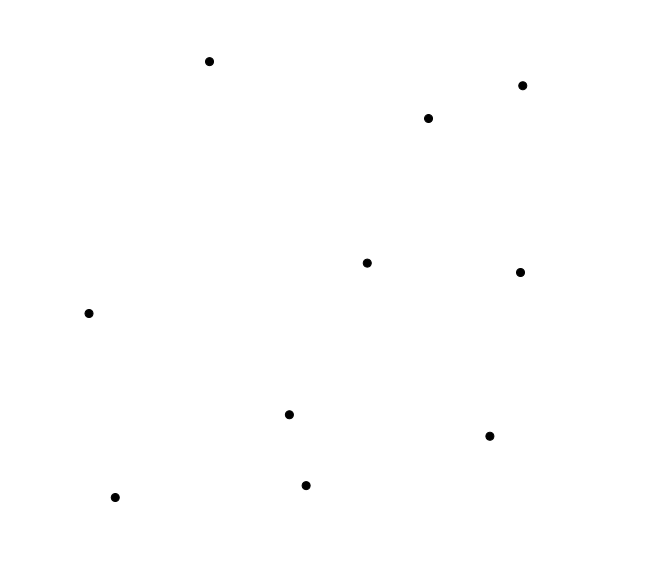
\includegraphics[width=\linewidth]{Figures/DTEx_a.png}
\caption{} \label{fig:DTEx_a}
\end{subfigure}
\hspace*{\fill} % separation between the subfigures
\begin{subfigure}{0.31\textwidth}
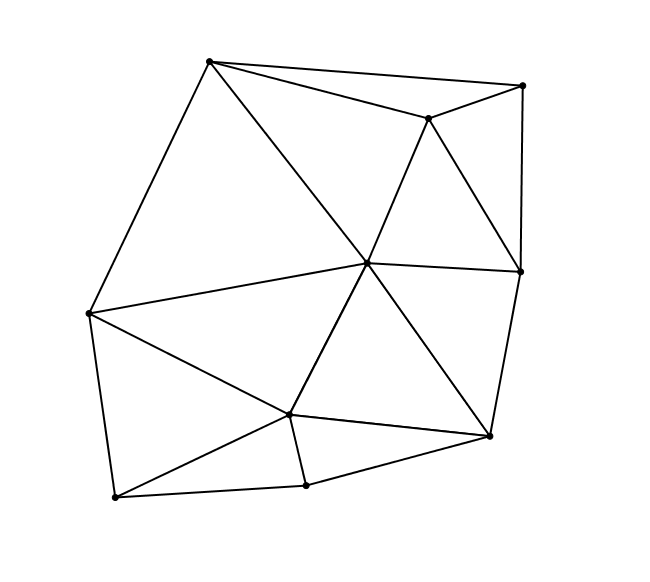
\includegraphics[width=\linewidth]{Figures/DTEx_b.png}
\caption{} \label{fig:DTEx_b}
\end{subfigure}
\hspace*{\fill} % separation between the subfigures
\begin{subfigure}{0.31\textwidth}
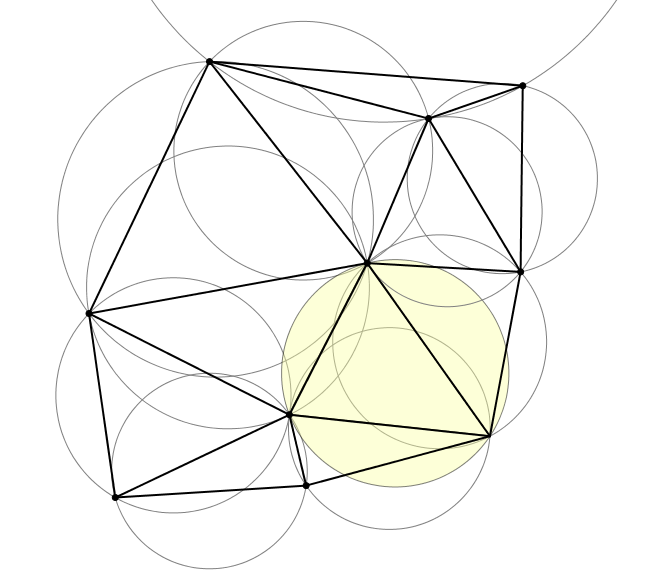
\includegraphics[width=\linewidth]{Figures/DTEx_c.png}
\caption{} \label{fig:DTEx_c}
\end{subfigure}
\caption[An example for the Delaney triangulation.]{An example for the Delaney triangulation.  In \ref{fig:DTEx_a}, a finite set of points is given. Its Delaunay triangulation is illustrated in \ref{fig:DTEx_b}. \ref{fig:DTEx_c} labels the circumscribed circle of every triangle in blue. Adapted from Wikipedia\cite{wiki:DT}.} \label{fig:DTEx}
\end{figure}



\section{ Stretch Factor}
The stretch factor $\rho$ of the Delaunay triangulation $D$ is the maximum ratio, among all points $p$ and $q$ in $S$, of the shortest path distance from p to q in $D$ over the Euclidean distance $\|pq\|$. The formula is provided as the following.
\[\rho(D) = \max_{\forall{p, q\in S}}\frac{{\min{|P(p, q)|}}}{||pq||}.\]

The concept of stretch factor have some other names such as dilation, spanning ratio or distortion.
In this thesis, we investigate the tight bound on the stretch factor of the Delaunay triangulation.  





\section{Arcgons}
We define a \textbf{disk} $d$ is the region in a Euclidean plane bounded by a circle $c$. 
Then,  a graph $f$ is  a \textbf{face} if its edges are the boundary of a convex subset of a disk $d$, and its vertices are on the boundary of $d$. 
Thus, the edges of a face is either circular arcs or straight lines. We say the circle $c$ is the \textbf{base circle} of the face $f$.

A \textbf{circles segment} is a region  bounded by an arc and the chord connecting the endpoints of the arc. Then, a \textbf{face on circle segment} is a graph whose edges are the boundary of a circle segment, and vertices are the two endpoints of the arc.


An \textbf{arcgon} is a planar graph defined as a finite sequence of distinct faces $F = \{f_1, f_2, \dots, f_n\}$ that meets the following conditions.
\begin{enumerate}

    \item The two ends $f_1$ and $f_n$ are faces on circle segment with a special vertex on the circular arc edge called  the \textbf{terminal point}. Denote the terminal points on $f_1$ and $f_n$  as $p$ and $q$ respectively. 
    \item For every two consecutive faces $f_i$ and $f_{i+1}$, $1\le i\le n-1$, none of the circular arcs of $f_i$ and $f_{i+1}$ intersects, and exactly one straight line edge of $f_i$ is also a straight line edge of $f_{i+1}$. Those interior straight line edges are called as \textbf{diagonals}.
    \item The union of regions bounded by all faces in $F$ has a boundary constructed by curricular arcs. That is, the outsider boundary contains only circular arc edges. 
    \item (Local Delaunay) Vertices of every  face $f_i$, $1\le i\le n-1$, lie either on or outside the base circles of neighboring faces $f_{i-1}$ and $f_{i+1}$.
    \item ($pq$-Delaunay) $p$ and $q$ are either on or outside all basic circles of faces in $F$.
    \item (Realizability) All diagonals intersect the segment $\overline{pq}$ at some points except their ends.
\end{enumerate}

Define the \textbf{stretch factor} of an arcgon $A$ as the ratio of the shortest path distance between the terminal points $p$ and $q$ over the their Euclidean distance $||pq||$. 


The definition of arcgons is well defined so that studying the tight bound on the stretch factor of arcgons is equivalent to studying on the the stretch factor of Delaney triangulation. Given a Delaunay triangulation of a point set, and suppose its stretch factor is $\rho$. Since the stretch factor of Delaney triangulation is defined as the max ratio over all pair of points, we can always choose a pair of some points $p$ and $q$ such that the ratio of their shortest path over their Euclidean distance is $\rho$ and none pairs of points has a ratio greater than that. Then, consider all triangles passed by $\overline{pq}$. Take their circumcircles as our base circle of faces. And construct an arcgon based on those faces. Then, the stretch factor of the arcgon is not less than $\rho$. That is, if we prove the stretch factor of an arcgon is at most $\kappa$, we can say that the stretch factor of a Delaney triangulation must be at most $\kappa$. 


The argument above shows an upper bound for the stretch factor of arcgons is an upper bound for that of Delaunay triangulation. On the other hand, since we can always convert an arcgons to a Delaunay triangulation, it is clear that a lower bound for the stretch factor of arcgons will be a lower bound for that of Delaunay triangulation. Therefore, since the tight bound for the stretch factor of arcgons is equivalent to that of Delaunay triangulation, we will focus on the arcgons instead in this thesis.




We say an edge $e$ of an arcgon is \textbf{critical} if there is a shortest path between $p$ and $q$ passing through $e$. If all edges in an arcgon is critical, the arcgon is a \textbf{critical arcgon}. 



An arcgon is \textbf{symmetric} if there is a line $l$ in the plane perpendicular to $pq$ such that the reflection of the arcgon with respective to $l$ is the same as the arcgon. Then, we say a \textbf{symmetric critical arcgon} is an arcgon if it is symmetric and critical.









\section{Applications}
The stretch factor of the Delaunay triangulation has wide applications.
\subsection{Network Design}
In 1989, Chew\cite{chew} mentioned that network design would an application.  Consider servers as vertices and channels between servers as edges. Then, using Delaunay triangulation to construct a network may close to give the optimal solutions. First, the network we develop in Delaunay triangulation is planar. Thus, only the linear number of edges are needed. This property could significantly reduce the complexity of problems relative to network. Also, the worst transmission distance between two sites are bounded. According to  the lower bound of the stretch factor shown in \cite{xia}, the shortest path distance between two servers would not be greater than $1.998$ times the physical distance.

In 2003, Li, Calinescu, Wan and Wang\cite{ad} the application of Delaunay triangulation in wireless computing, in particular, ad hoc wireless networks. An ad hoc  wireless network is a type of computer-to-computer connection. Users do not need to connect with Wi-Fi to communicate with each other. That is, a computer can build up a wireless connection directly to another computer. If the built-in network topology is the Delaunay triangulation, some localized routing protocols will guarantee the delivery of the packets. Then, the total distance traveled by the packet over the physical distance is our stretch factor. Therefore, improving the bound on the stretch factor of the Delaunay triangulation will directly prove the performance of wireless computing. 





\subsection{Motion Planning Problem}
A motion planning problem is to find the best path moving from a start configuration  $S$ to a goal configuration $G$, while avoiding collision with known obstacles. Chew \cite{chew} discussed the connection between this problem and Delaunay triangulation, in particular,  the constrained Delaunay triangulation. A constrained Delaunay triangulation is a generalization of the Delaunay triangulation that forces certain required segments into the triangulation. Figure~\ref{fig:CDT} gives a comparison between an ordinary Delaunay triangulation and a constrained Delaunay triangulation. 



\begin{figure}[ht]
\centering
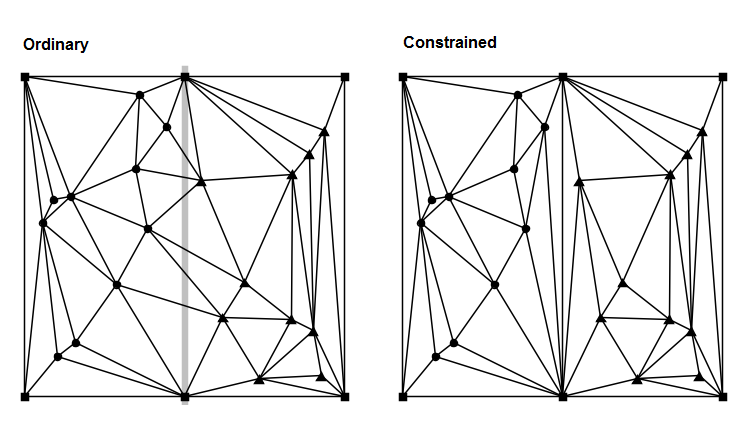
\includegraphics[width=80mm]{Figures/CDT.png}
\caption[A Delaunay triangulation and a constrained Delaunay triangulation.]{A Delaunay triangulation and a constrained Delaunay triangulation. The  ordinary one on the left hand side is a Delaunay triangulation. Suppose there is an obstacle in the middle of the graph as shown in gray. Our triangulation is constrained, and there must be a edge in the place of the obstacle. Reprinted form \cite{github}.} 
\label{fig:CDT}
\end{figure}

Constrained Delaunay triangulation is largely applied in the field of topographic surveying. Consider there is a river crosses some edges in the triangulation based on a city. That is, the original designed paths do not accurately describe the path of the river. Then, by adding the river as a breakline in the triangulation, the graph could better model the possible paths between vertices. Anderson, Karumanchi and Iagnemma explained the application of constrained Delaunay triangulation in semi-autonomous vehicles. Figure~\ref{fig:auto} shows the model of path planning using constrained Delaunay triangulation.

\begin{figure}[ht]
\centering
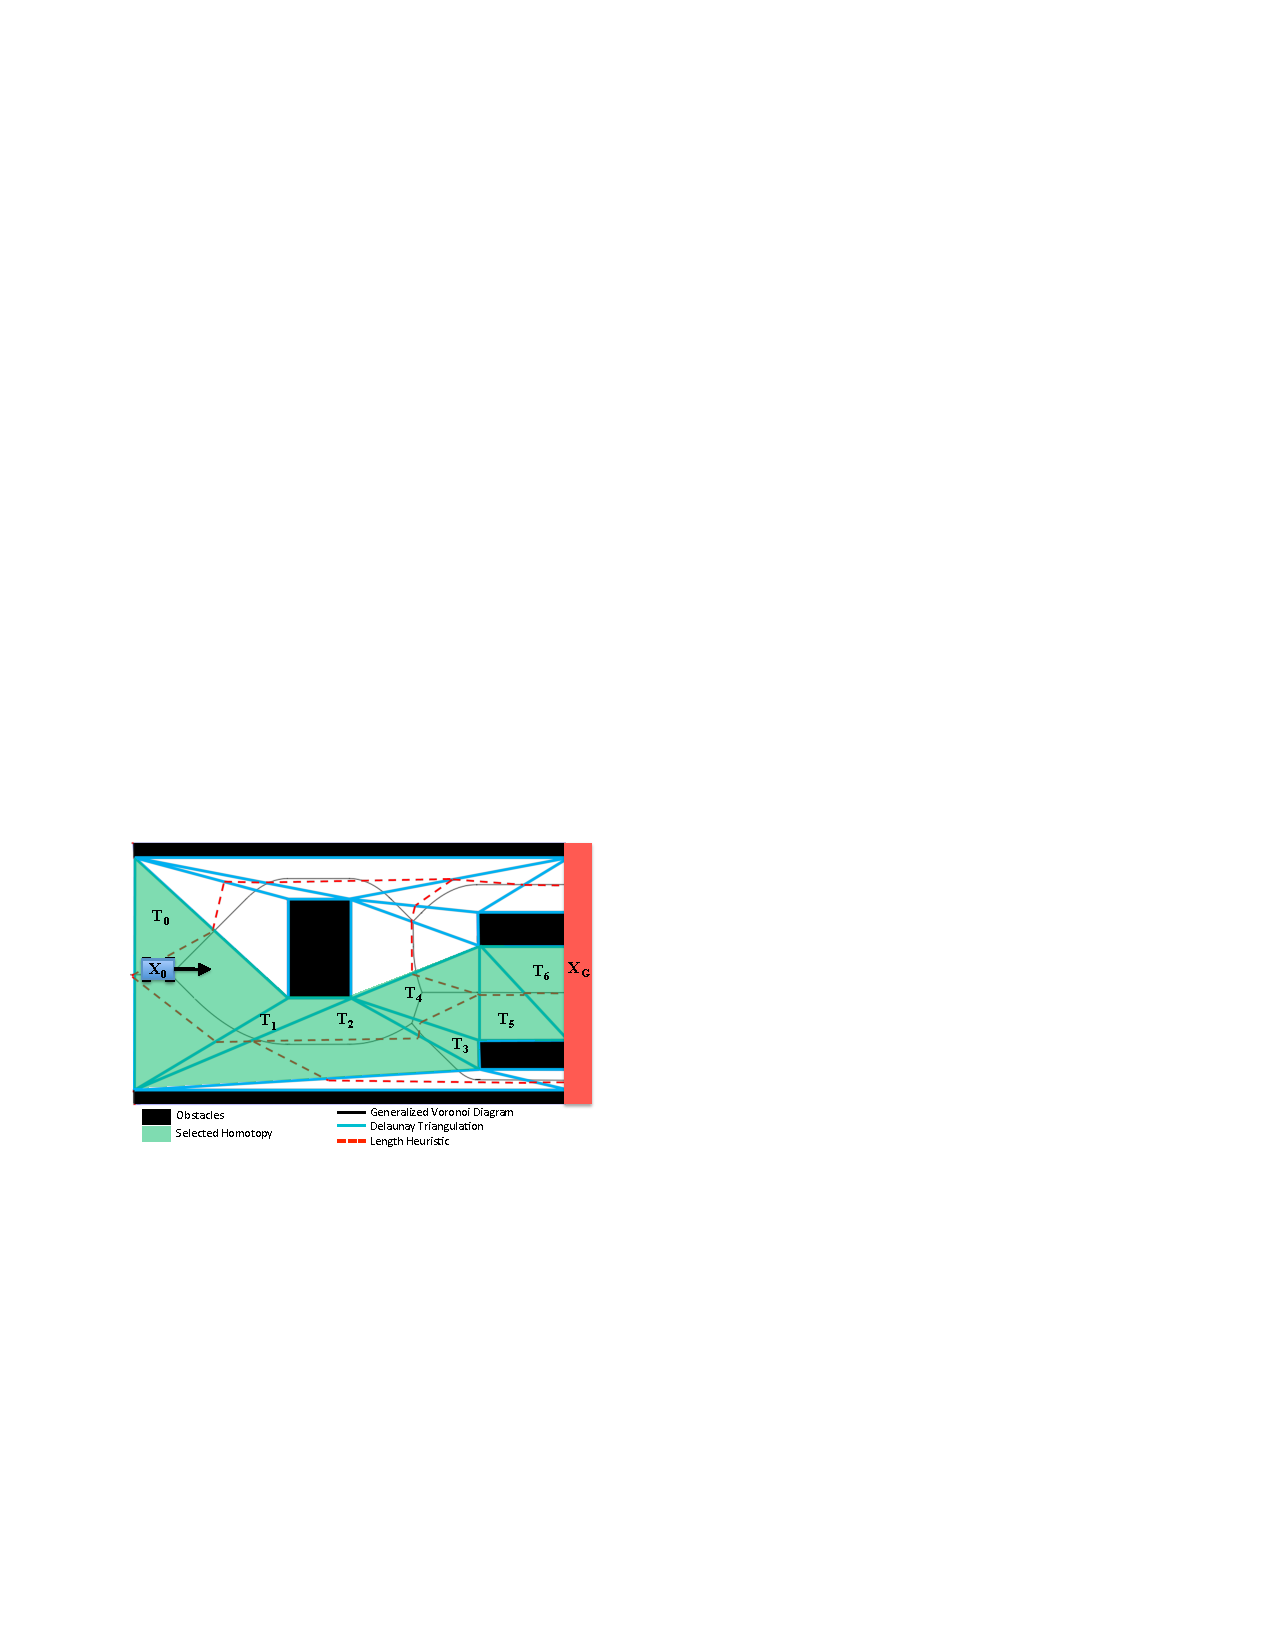
\includegraphics[width=100mm]{Figures/auto.pdf}
\caption[Constrained Delaunay triangulation in path planning in Automated driving]{Constrained Delaunay triangulation in path planning in Automated driving. Reprinted form \cite{auto}.} 
\label{fig:auto}
\end{figure}




\section{Organization of the Thesis}
In this thesis, we focus on the stretch factor of a special case in Delaunay triangulation, the symmetric critical arcgon. In section 3, we derive formula for our basic case, the stretch factor of symmetric critical arcgons with three circles. Section 4 gives a general formula. Then, we attempt to improve both the lower and upper bounds. section 5 illustrates how we show the existence of some worse stretch factor with the general formula in section 3. And section 6 provides a complete proof showing that an upper bound of stretch factors for all symmetric critical arcgons with  three circles is $1.6$. 
\chapter{Literature Review}
The problem of proving a tight bound on the stretch factor of the Delaunay triangulation has received considerable attention in the area of computational geometry. And there is a long list of results on improving both the lower and upper bounds.

% \textcolor{blue}{(Maybe add a graph as a timeline for both lower bound & upper bound, but in what form (arrows, direction, ...)? Or, too many figures?)}

\section{On the Lower Bound}

\subsection{\texorpdfstring{$\pi/2\approx 1.5708$}     {Lg}, Chew in 1989}

As we mentioned in section 1.2, the property stretch factor of Delaunay triangulation was first introduced by Chew\cite{chew} in 1987. Although the main result was on TD (triangle distance) Delaunay triangulation, Chew discussed the stretch factor in the case of standard Delaunay triangulation at the end of the paper. Chew pointed out it was clear that $\pi/2$ is a lower bound by constructing a set of points on a unit circle. 

Bose et al.\cite{BoseCGTA} wrote a rigor proof based on Chew's idea and gave a detailed illustration as Figure~\ref{fig:pi:2}. We first distribute a set of points uniformly on a unit circle. Choose two points $p$ and $p'$ that are diametrically opposite with each other. Then, let us construct a triangulation with all edges which are nearly perpendicular to $\overline{pp'}$. Since all points are on the same circle, the triangulation must be a Delaunay triangulation. Also, for every pair of points, the shortest path should be the one along the boundary of the circle. Therefore, as the set of points become larger, the ratio for the pair of $p$ and $p'$ approaches $\pi/2$, and that ratio is always the maximum among all pairs. Thus, the stretch factor would be close to $\pi/2$.

\begin{figure}[ht]
\centering
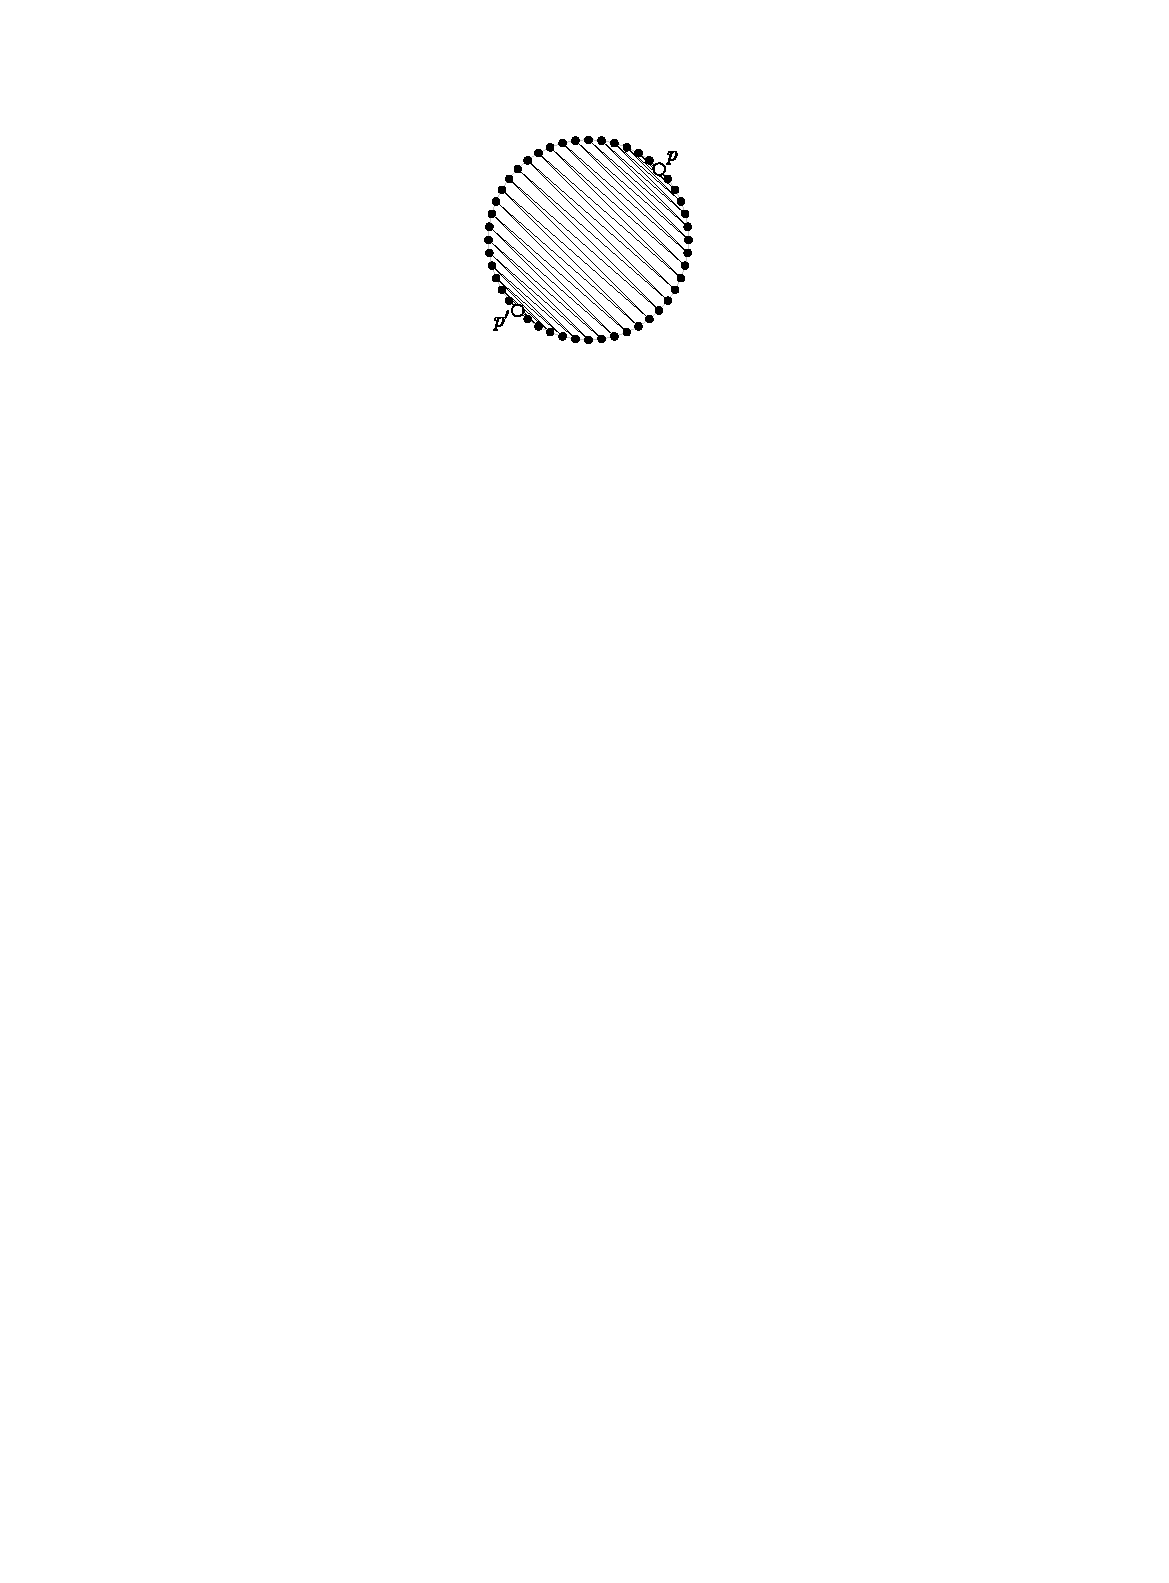
\includegraphics[width=50mm]{Figures/pi:2.pdf}
% \decoRule
\caption[An instance that the stretch factor approaches $\pi/2$]{An instance that the stretch factor approaches $\pi/2$. Reprinted from Bose et al.\cite{BoseCGTA}.} 
\label{fig:pi:2}
\end{figure}









\subsection{\texorpdfstring{$1.5846$}{Lg}, Bose et al. in 2009}
It has long been conjectured that the lower bound of stretch factor can be at most $\pi/2$ until Bose et al. \cite{BoseCGTA} constructed a point set with the  stretch factor great than 1.5846 in 2009.
Their construction is based on the following  observation. Consider a sector of a unit circle as in Figure~\ref{fig:Bose_a}. According to the figure, there are two types of locally optimal path from $p$ to $q$: 1)the arc $pq$  around the sector, and 2) the path consisting of the arc $pq'$ followed by the segment $q'q$. Bose et al. proved that when $\beta$ under a certain condition relative to $\theta$,  path 1 is shorter than path 2. Thus, if we can make every $\beta$ meet the appropriate condition, the observation would guarantee the path along the perimeter as the shortest. The paper provided a model made up two unit semicircles with a gap $d$. Figure~\ref{fig:Bose_c} is a construction with a stretch factor of $1.5810$. 

Bose et al. stated that  the instance in Figure~\ref{fig:Bose_c} is valid for a set of points in convex position, which is a more general definition comparing with that in plane. Also,  they claimed they could increase the stretch factor slightly by replacing the two straight segments with points on a common circle $C$ and adding four shield points $s$. (Figure~\ref{fig:Bose_d}) Then, no edges inside the polygon is used. And the lower bound of stretch factor for points in the plane was improved to be $1.5846$.



\begin{figure}[ht]
        \centering
        \begin{subfigure}[b]{0.475\textwidth}
            \centering
            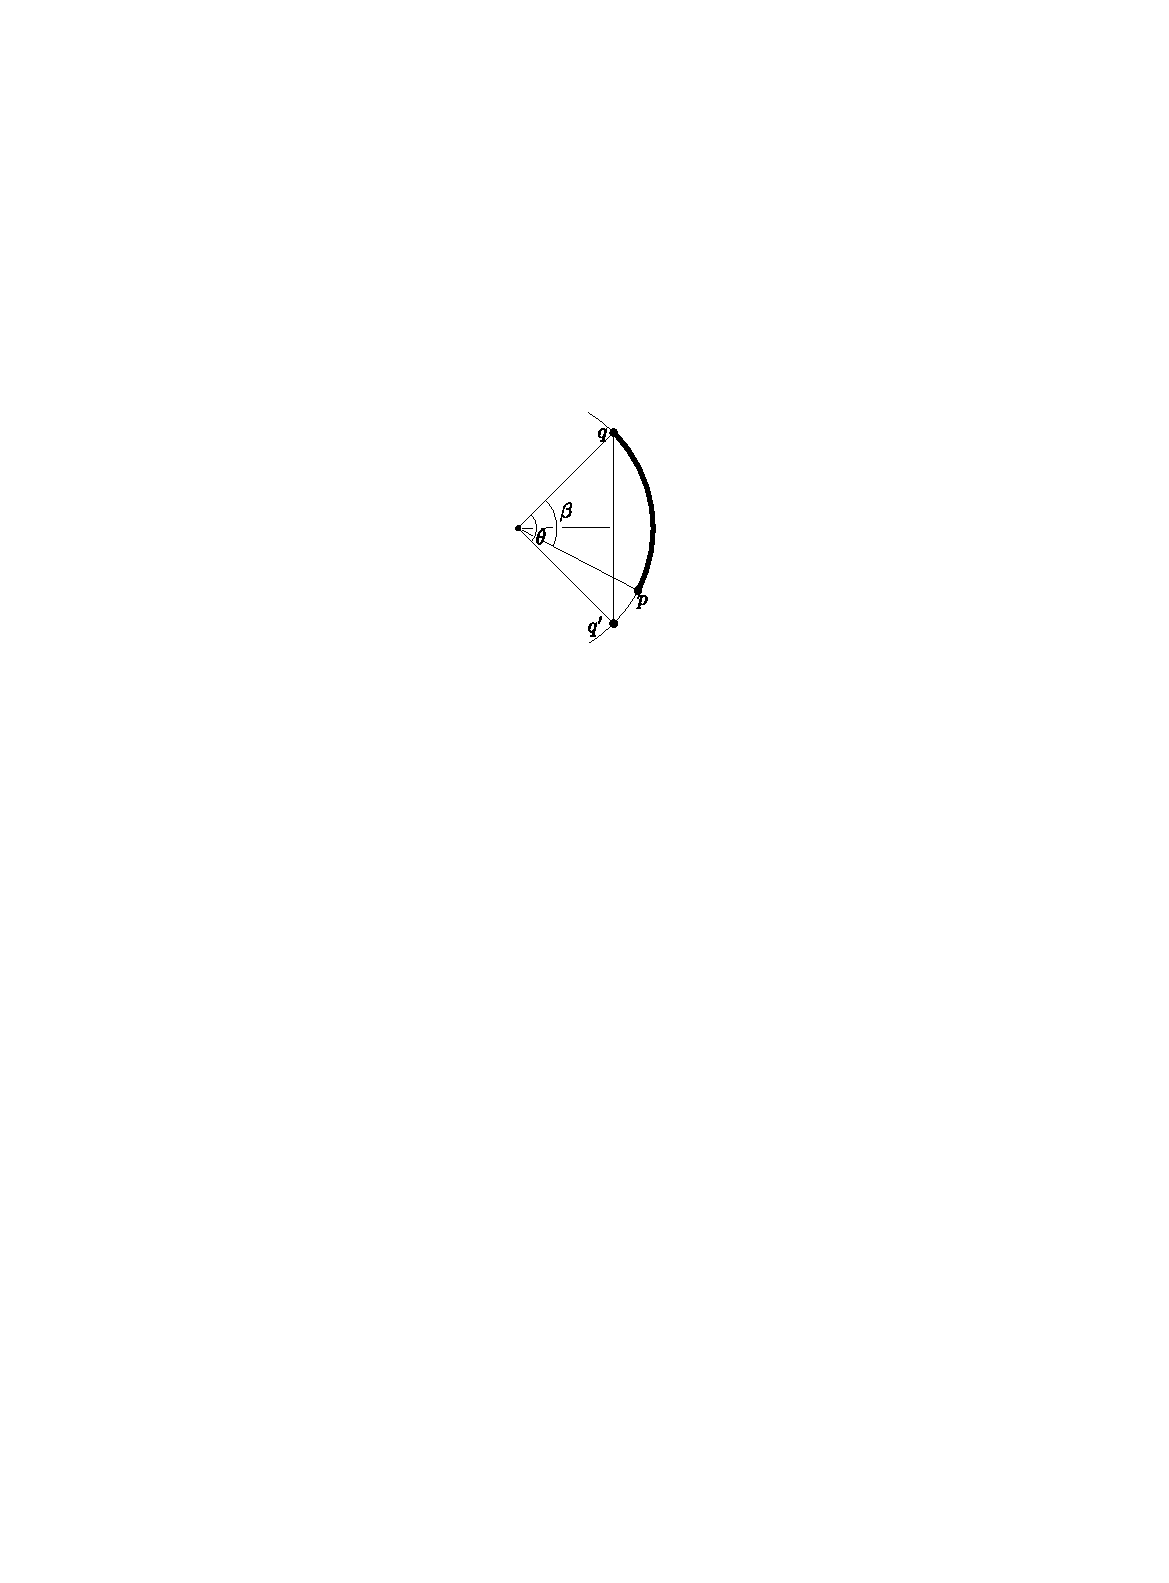
\includegraphics[width=.8\textwidth]{Figures/Bose_a.pdf}
            \caption[]%
            {{}}    
            \label{fig:Bose_a}
        \end{subfigure}
        \hfill
        \begin{subfigure}[b]{0.475\textwidth}  
            \centering 
            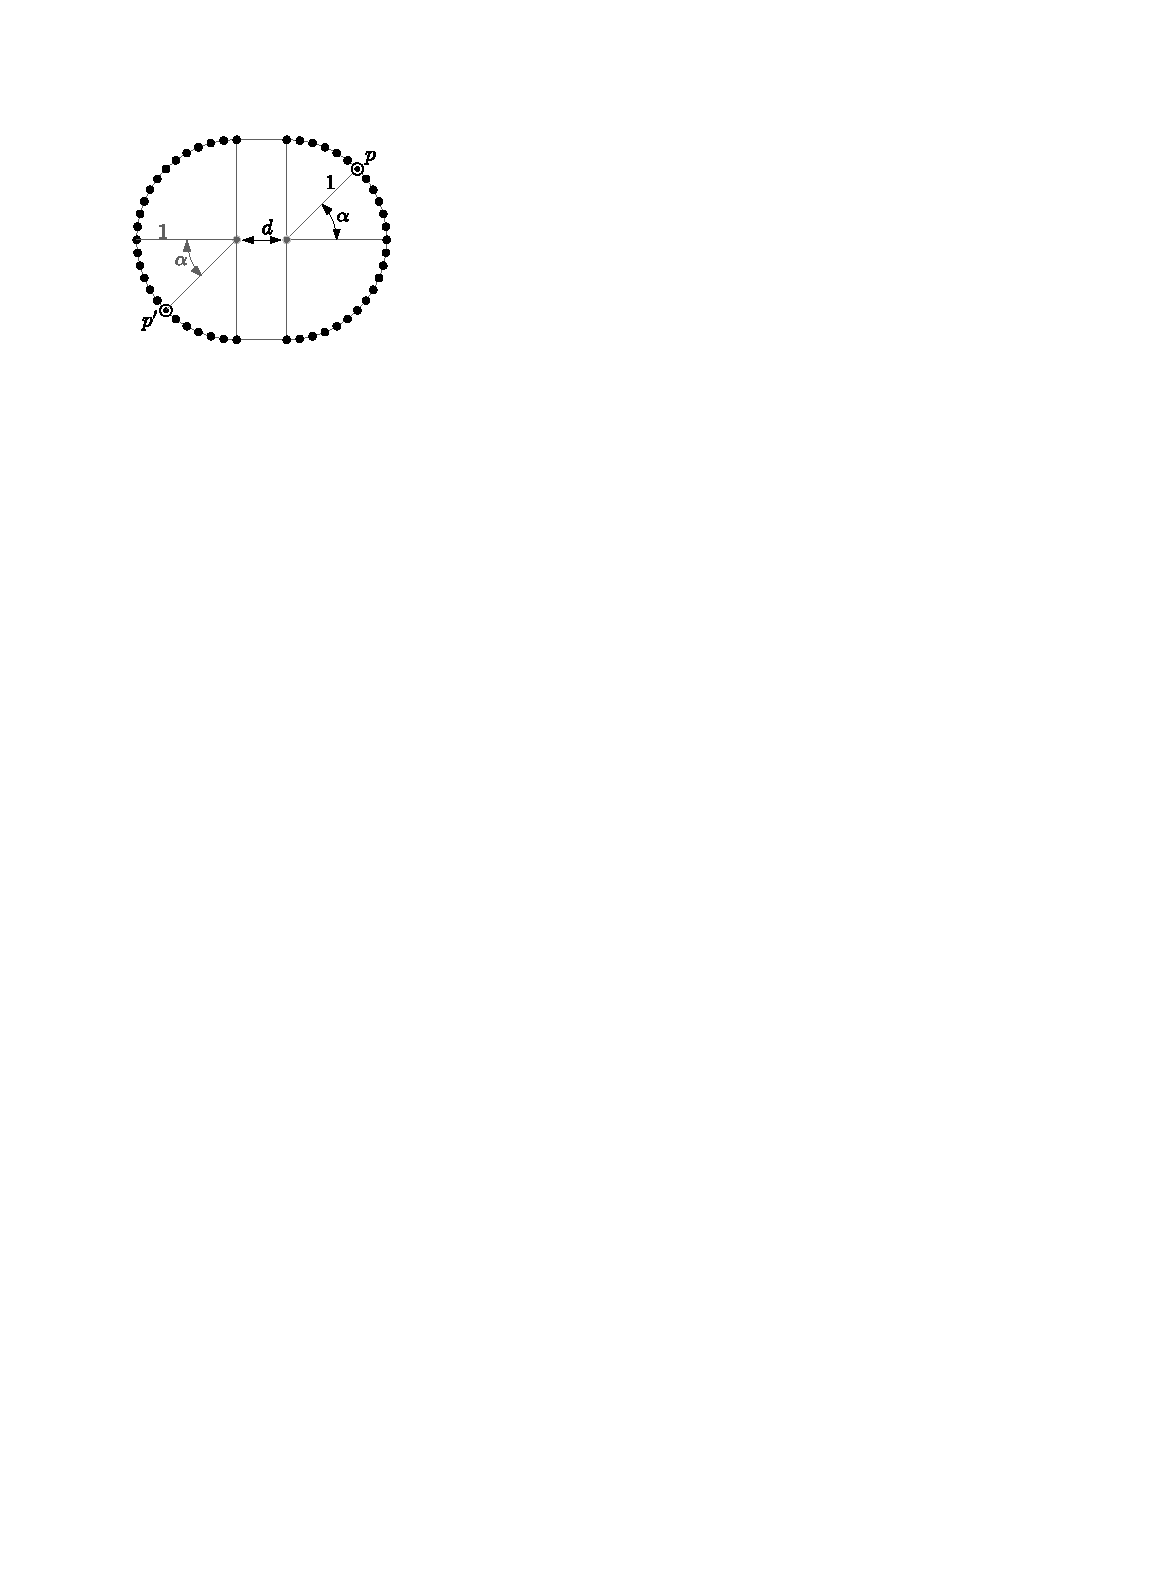
\includegraphics[width=.8\textwidth]{Figures/Bose_b.pdf}
            \caption[]%
            {{}}    
            \label{fig:Bose_b}
        \end{subfigure}
        \vskip\baselineskip
        \begin{subfigure}[b]{0.475\textwidth}   
            \centering 
            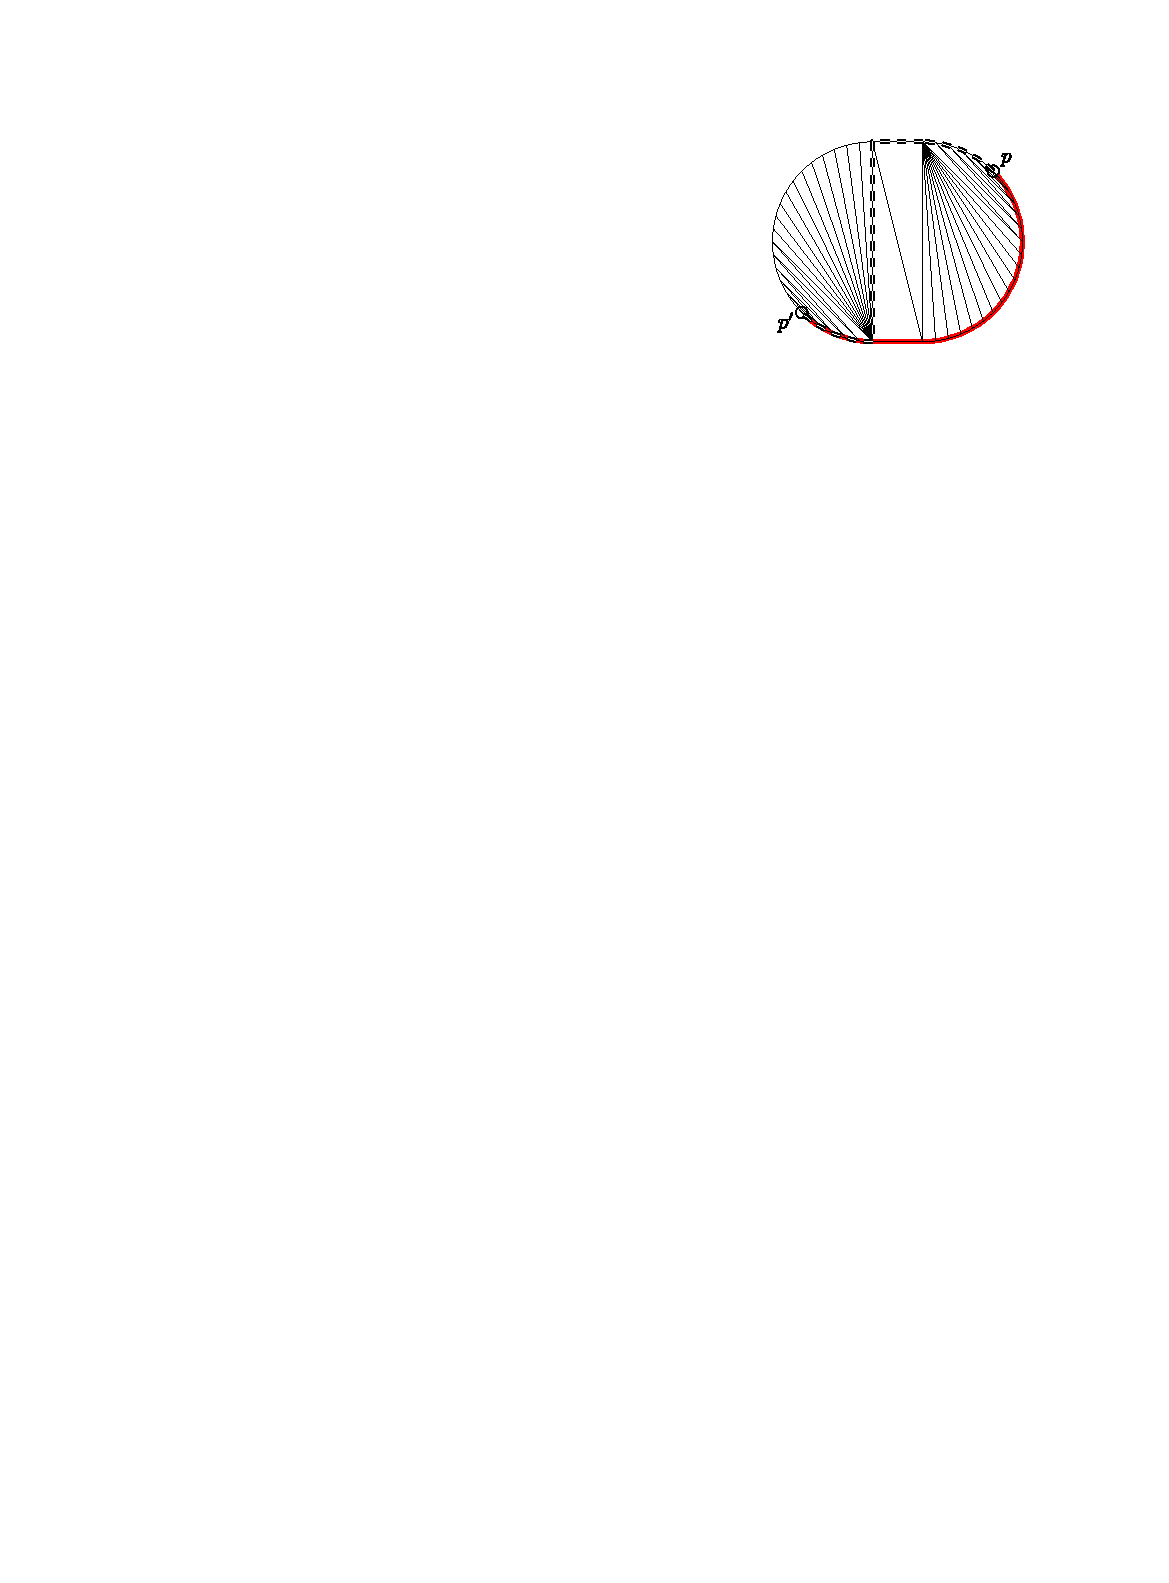
\includegraphics[width=.8\textwidth]{Figures/Bose_c.pdf}
            \caption[]%
            {{}}    
            \label{fig:Bose_c}
        \end{subfigure}
        \quad
        \begin{subfigure}[b]{0.475\textwidth}   
            \centering 
            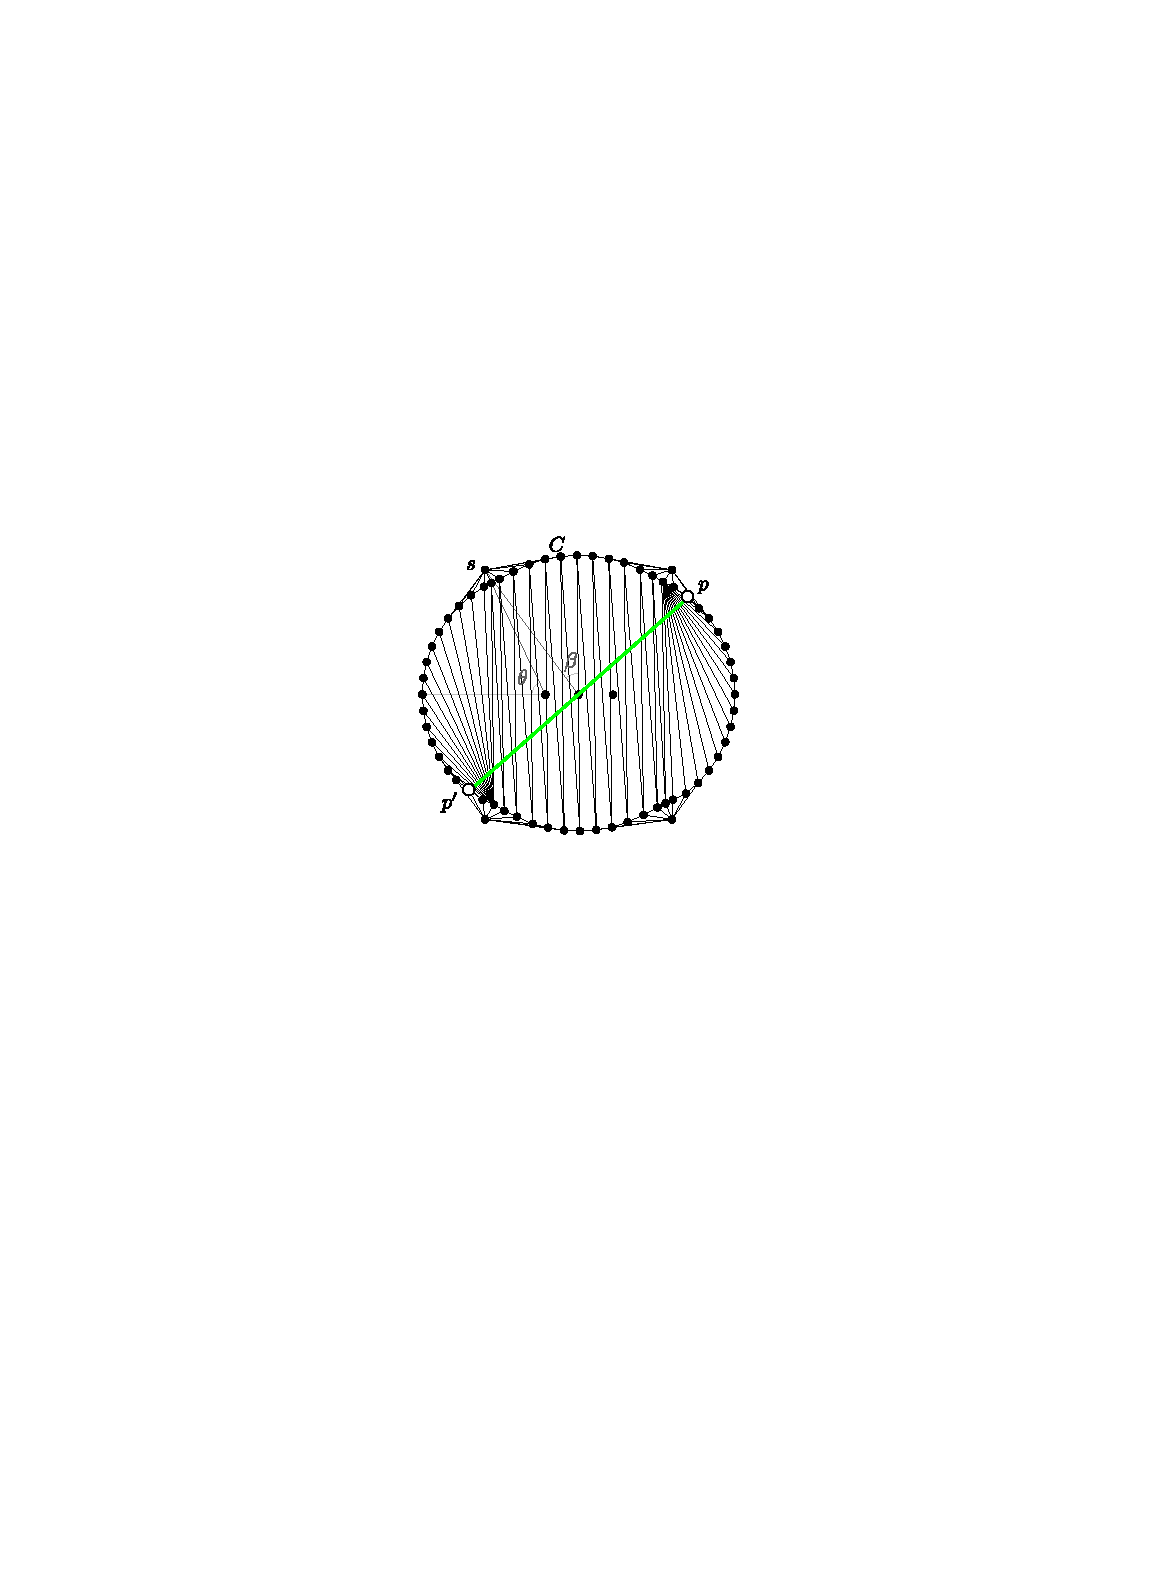
\includegraphics[width=.8\textwidth]{Figures/Bose_d.pdf}
            \caption[]%
            {}    
            \label{fig:Bose_d}
        \end{subfigure}
        \caption[Illustrations for the model proving a lower bound 1.5846]{Illustrations for the model proving a lower bound 1.5846. \ref{fig:Bose_a} illustrates two types of locally optimal paths from $p$ to $q$.  \ref{fig:Bose_b} and  \ref{fig:Bose_c} give the construction for point set in convex position, a more general case comparing with the topic we study.  \ref{fig:Bose_d} is the instance with a stretch factor of 1.5846. Reprinted from \cite{BoseCGTA}.} 
        \label{fig:Bose}
    \end{figure}





\subsection{\texorpdfstring{$1.5932$}{Lg}, Xia and Zhang in 2011}
Xia and Zhang\cite{fwcg2010} improved the lower bound to  $1.5932$ in  2011 by reducing the problem to studying the stretch factor of a family of chains satisfying certain structural properties. According to  \cite{dobkin}, we know that the maximum stretch factor among all chains made by $n+1$ circles is always greater than the maximum stretch factor among claims with  $n$ circles. Thus, they aimed to establish a well-defined family of chains such that every chain has the maximum stretch factor among all chains made by the same number of circles.
Figure~\ref{fig:ZX} gives an illustration of the chains with worse bounds.




\begin{figure}[ht]
\hspace*{\fill}
\begin{subfigure}{0.45\textwidth}
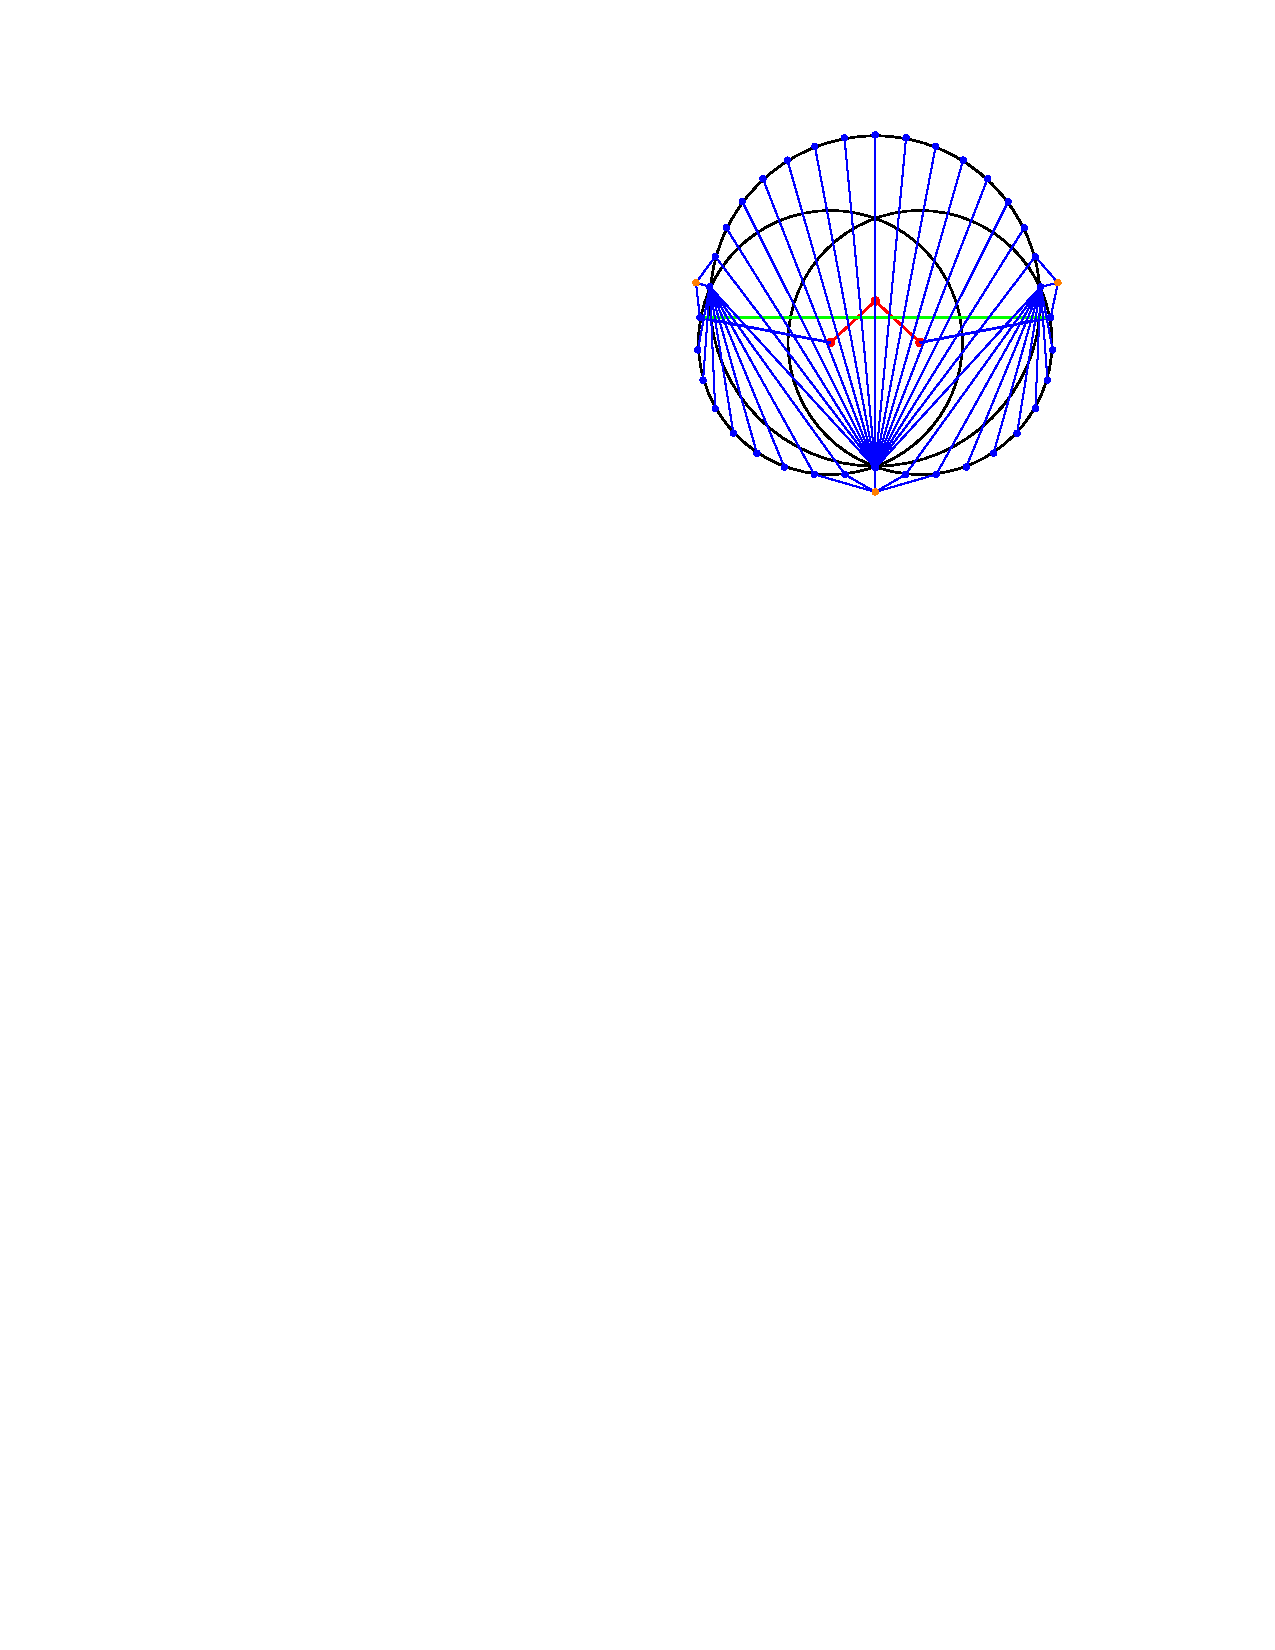
\includegraphics[width=\linewidth]{Figures/ZX_3.pdf}
\caption{} \label{fig:ZX_3}
\end{subfigure}
\hspace*{\fill} % separation between the subfigures
\begin{subfigure}{0.45\textwidth}
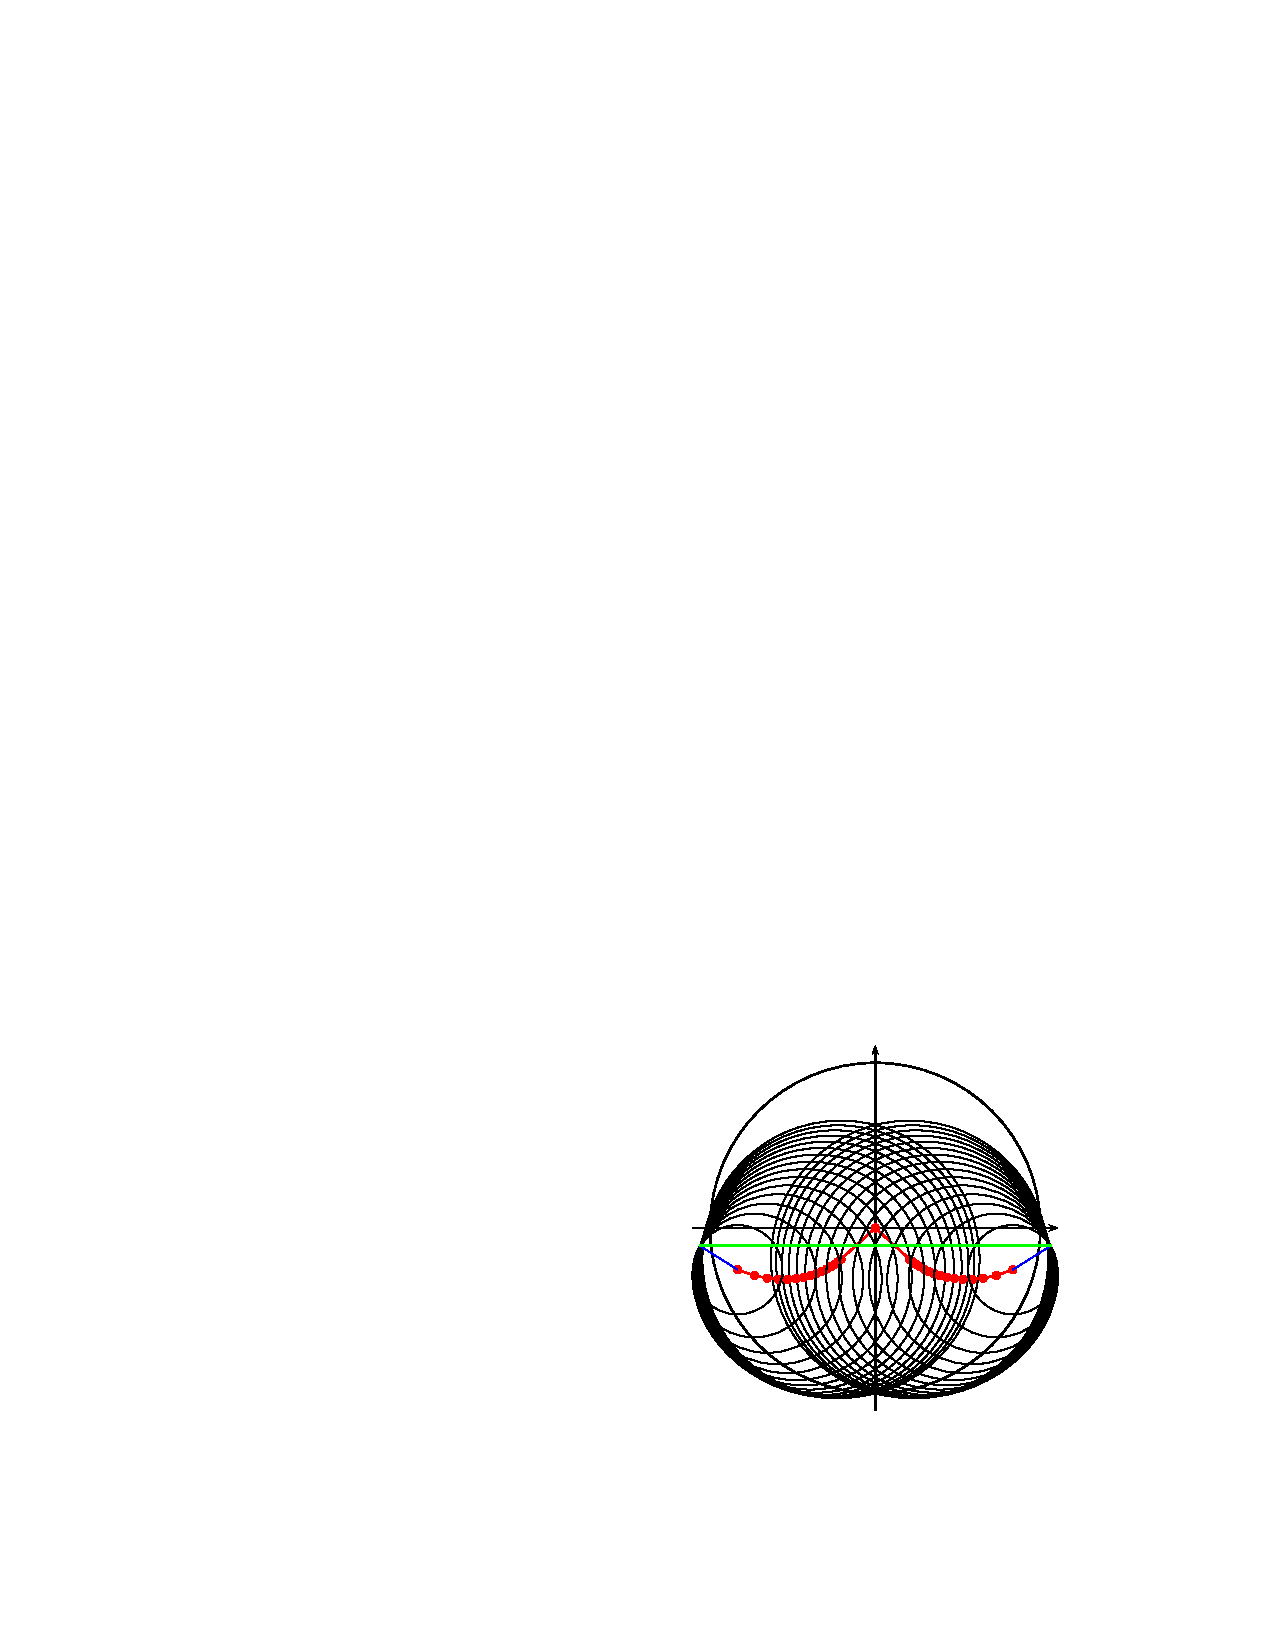
\includegraphics[width=\linewidth]{Figures/ZX_31.pdf}
\caption{} \label{fig:ZX_31}
\end{subfigure}
\hspace*{\fill}
\caption[A chain of circles with the stretch factor $1.5932$]{An instance for stretch factor $1.5932$. \ref{fig:ZX_3} shows shield points and edges in the basic case, a chain of three circles. \ref{fig:ZX_31} is a chain of circles with stretch factor $1.5932$. Reprinted from \cite{fwcg2010}.} \label{fig:ZX}
\end{figure}








\subsection{\texorpdfstring{$1.59324$}{Lg}, Snoeyink and Verma in 2012}
Snoeyink and Verma used a  characterization to bring both upper and lower bounds closer to 1.6 in \cite{arcgon}. Instead of converting a point set into a chain of circles, they transformed the original model to a class of graphs called arcgon. Basically, an arcgon is an embedded graph made up by three types of faces shown  Figure~\ref{fig:SV}. An arcgon is similar with a chain of circles in \cite{fwcg2010}, but this definition makes them characterize edges more convenient. They conjectured that if a arcgon has the greatest stretch factor among all arcgons with the same faces, every path should be the shortest path. That is, every path has the same length. For the lower bound part, they constructed a arcgon following their conjecture and stated its stretch factor  is $1.5846$. But they did not provided the exact parameters in this paper. 







\begin{figure}[ht]
\centering

\includegraphics[width=100mm]{Figures/SV.pdf}
% \decoRule
\caption[Tree types of faces in arcgons]{Tree types of faces in arcgons. Reprinted from \cite{xia}.} 
\label{fig:SV}
\end{figure}






\section{On the Upper Bound}

\subsection{\texorpdfstring{$5.08$}{Lg},  Dobkin, Friedman, and Supowit in 1987}
The upper bound for the stretch factor was first shown by Dobkin, Friedman, and Supowit. They proved that all stretch factor of the Delaunay triangulation is at most $5.08$.  illustrates two types of paths from one end point on the $x$-axis $a$ to the other end point $b$. The path in Figure~\ref{fig:DFS_a} is called one-sided because all its intermediate points $b's$ are on one side of the $x$-axis. Then, since the length of the one-sided path from $a$ to $b$ could not be longer than the perimeter of the semicircle with a diameter $ab$, its stretch factor is at most $\pi/2$. 

We may also meet a case that the path is not even close to being ones-sided. For example, the path in Figure~\ref{fig:DFS_b} goes below the $x$-axis after $b_1$ and comes back to the positive range after $b_4$. For all such cases, Dobkin, Friedman and Supowit showed that the path length is at most $(1+\sqrt{5})$ times of the horizontal distance. Therefore, summing over all those sub-paths  would give a total path length at most $((1+\sqrt{5})/2)\pi$ times of  the distance. Therefore, they concluded the stretch factor of the Delaunay triangulation is at most $((1+\sqrt{5})/2)\pi\approx 5.08
$.




\begin{figure}[ht]
\begin{subfigure}{0.48\textwidth}
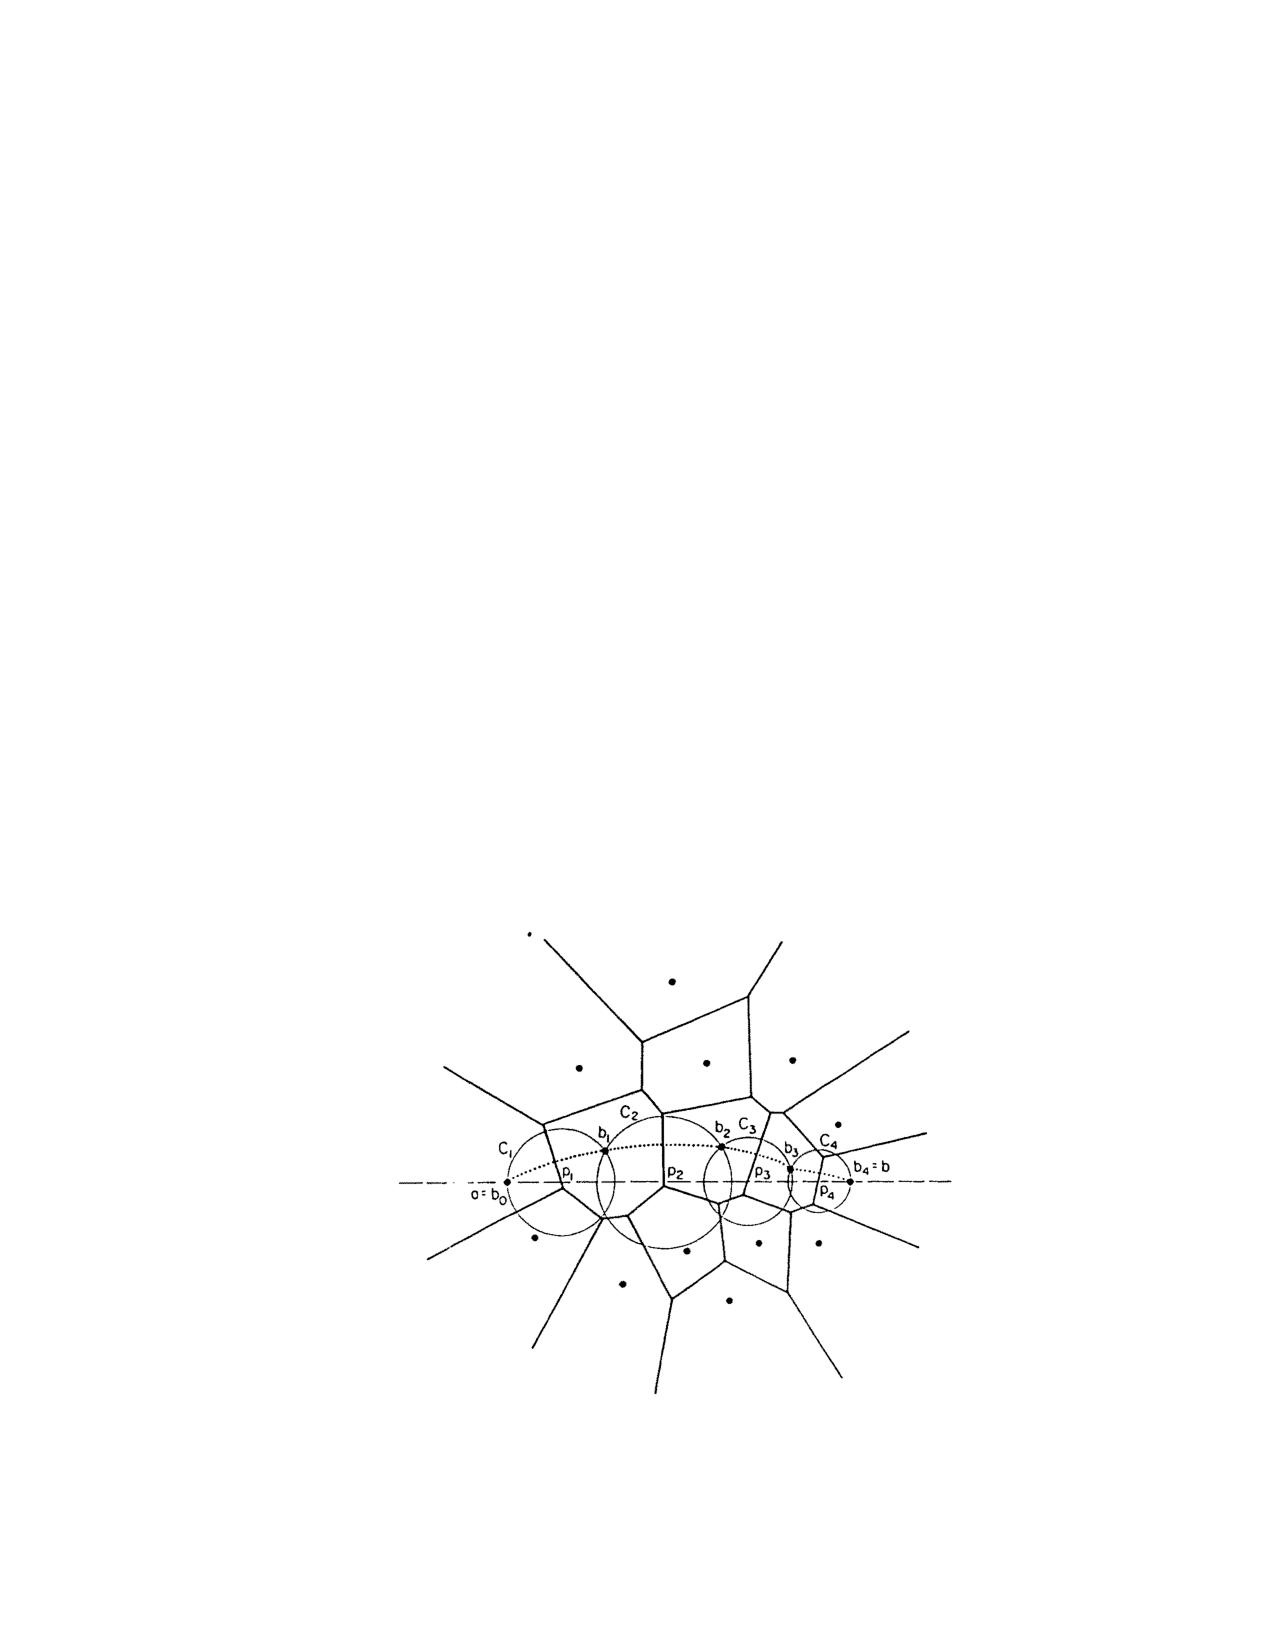
\includegraphics[width=\linewidth]{Figures/DFS_a.pdf}
\caption{} \label{fig:DFS_a}
\end{subfigure}
\hspace*{\fill}
\begin{subfigure}{0.48\textwidth}
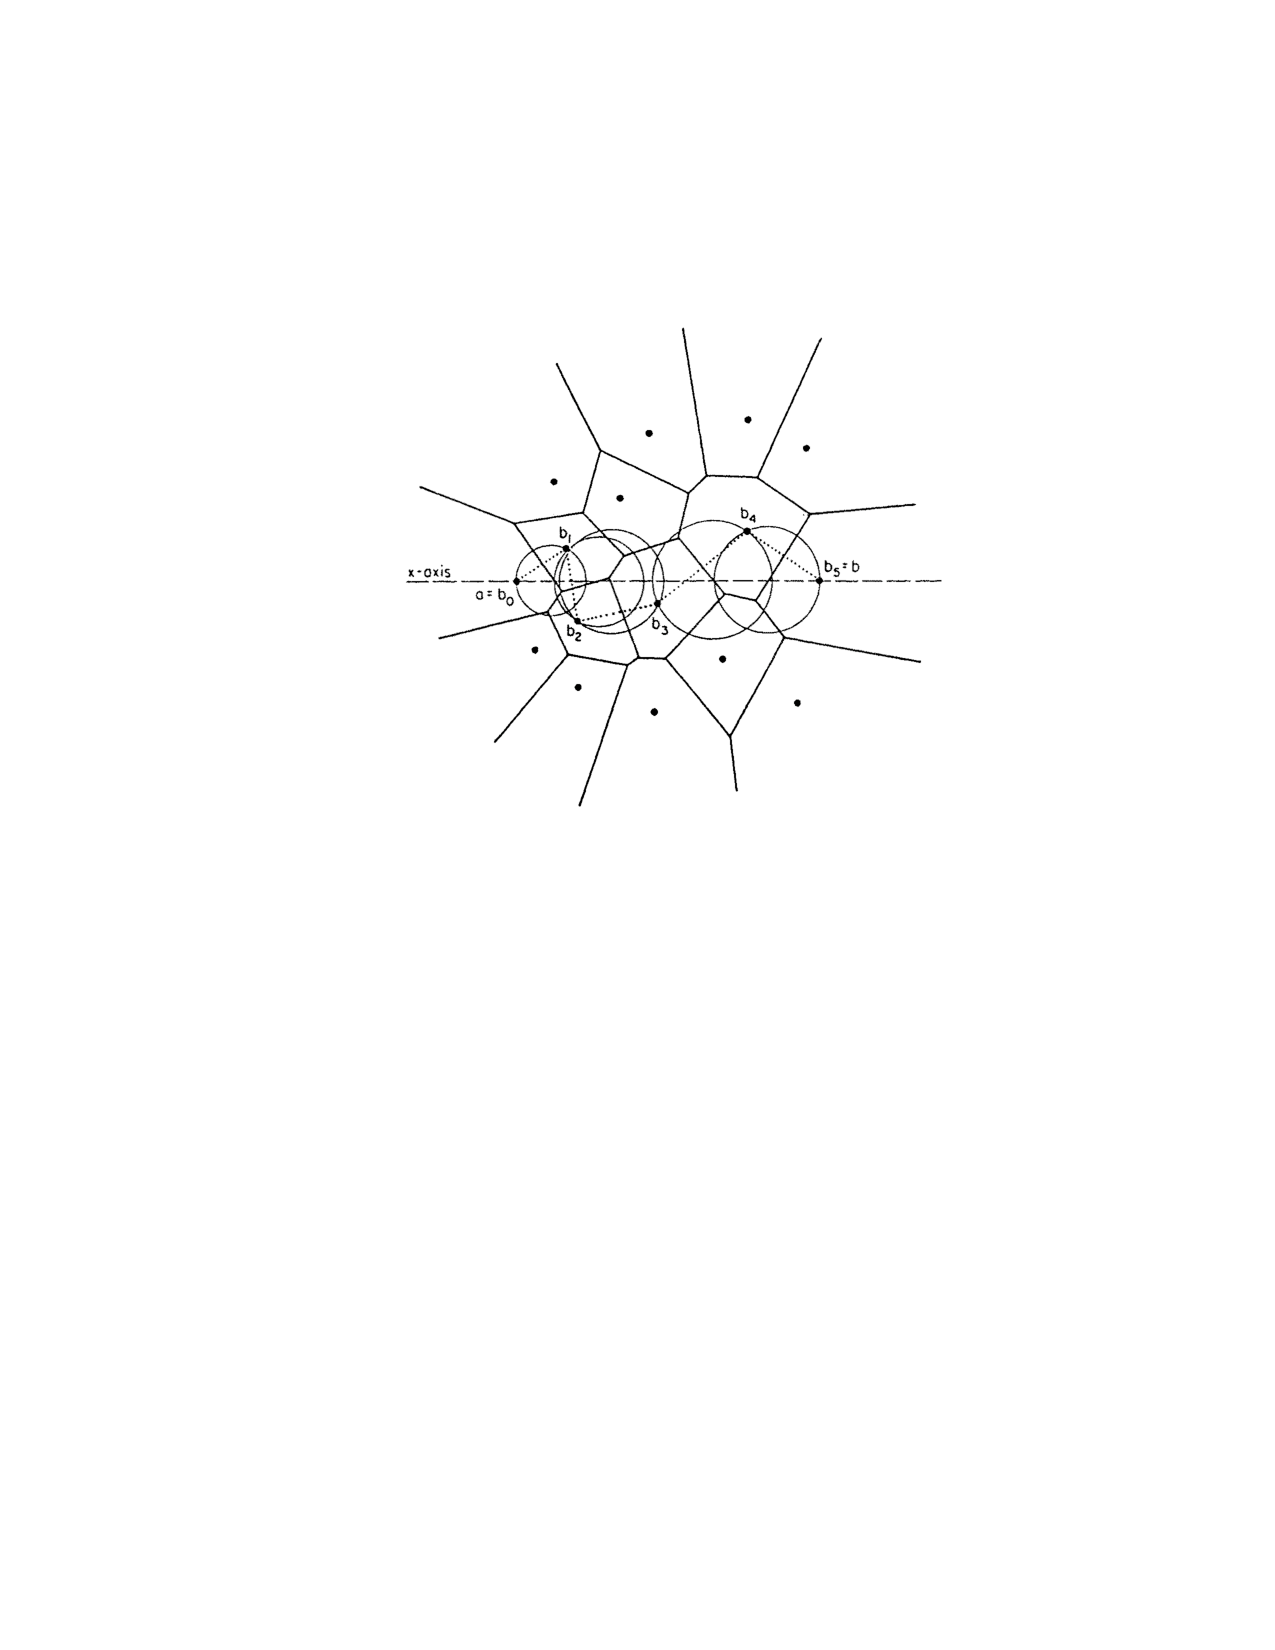
\includegraphics[width=\linewidth]{Figures/DFS_b.pdf}
\caption{} \label{fig:DFS_b}
\end{subfigure}
\hspace*{\fill} % separation between the subfigures
\caption[A one-sided path and a non one-sided path]{One-sided path and non one-sided path. Reprinted from \cite{dobkin}.} \label{fig:DFS}
\end{figure}


\subsection{\texorpdfstring{$2.42$}{Lg},  Keil and Gutwin in 1989}  
In 1989,  Keil and Gutwin published a paper\cite{keil} to discuss two classes of graphs which approximate the complete graph. One is the graph of the Delaunay triangulation. By analyzing they proved an upper bound of $2.42$. 

\subsection{\texorpdfstring{$1.998$}{Lg},  Xia in 2011}  
An upper bound of $1.998$ was shown by Xia\cite{xia} in 2011 with a different approach from the previous work. This approach in based on the geometry of a chain of disks in the plane. Then, by carefully defining the stretch factor of a chain in analogy to that of  the Delaunay triangulation, one could prove bound on the stretch of the Delaunay triangulation in the model of chains. After converting the Delaunay triangulation problem to a chain of disks, Xia proceeded the inductive proof by amortized analysis.  



\subsection{\texorpdfstring{$1.636245$}{Lg} (Conjectured), Snoeyink and Verma in 2012}
As we mentioned in section 2.1.4, Snoeyink and Verma stated a conjecture that  a arcgon which has the greatest stretch factor among arcgons with the same faces must have equal length paths. They proved that the upper bound could be improved to $1.636245$ once the conjecture is shown.
\chapter{Preliminaries}


\section{Notations}
In the following sections, we will express the points in the Euclidean plane in lowercase letters. For example, when we defined terminal points in section 1.3, we used lowercase letters $q$ and $p$. Also, we  may need  the notations for segments, rays and lines in definitions, theorems or proofs. Here are some rules for them. A segment $\overline{ab}$ is a straight line segment from the point $a$ to the point $b$. A ray from $a$ to $b$ is denoted as $\overrightarrow{ab}$. And a line $ab$ means a line passing though $a$ and $b$. An angle donation $\angle aob$ means an angle from ray $\overrightarrow{oa}$ to  ray $\overrightarrow{ob}$ in the counterclockwise direction. 






\section{Chains}
\begin{definition}
We define a finite sequence of distinct disks $\mathcal{O} = (O_1, O_2, \dots, O_n)$ be a \textbf{chain} if
\begin{enumerate}
    \item for $1\le i \le n-1$, every two consecutive disk $O_i$ ad $O_{i+1}$ intersect but do not contain each other. Then, for every disks $O_i$, define the \textbf{connecting arcs} of $O_i$ as the arcs on the boundary of $O_i$ in $O_{i-1}$  and in $O_{i+1}$, and denote as $C_{i}^{i-1}$ and $C_{i}^{i+1}$ respectively;
    \item The connecting arcs $C_{i}^{i-1}$ and $C_{i}^{i+1}$ for $2\le i\le n-1$ can share an endpoint but they do not overlap.
\end{enumerate}
\end{definition}


\begin{figure}[ht]
\centering
\begin{subfigure}{.8\textwidth}
\centering
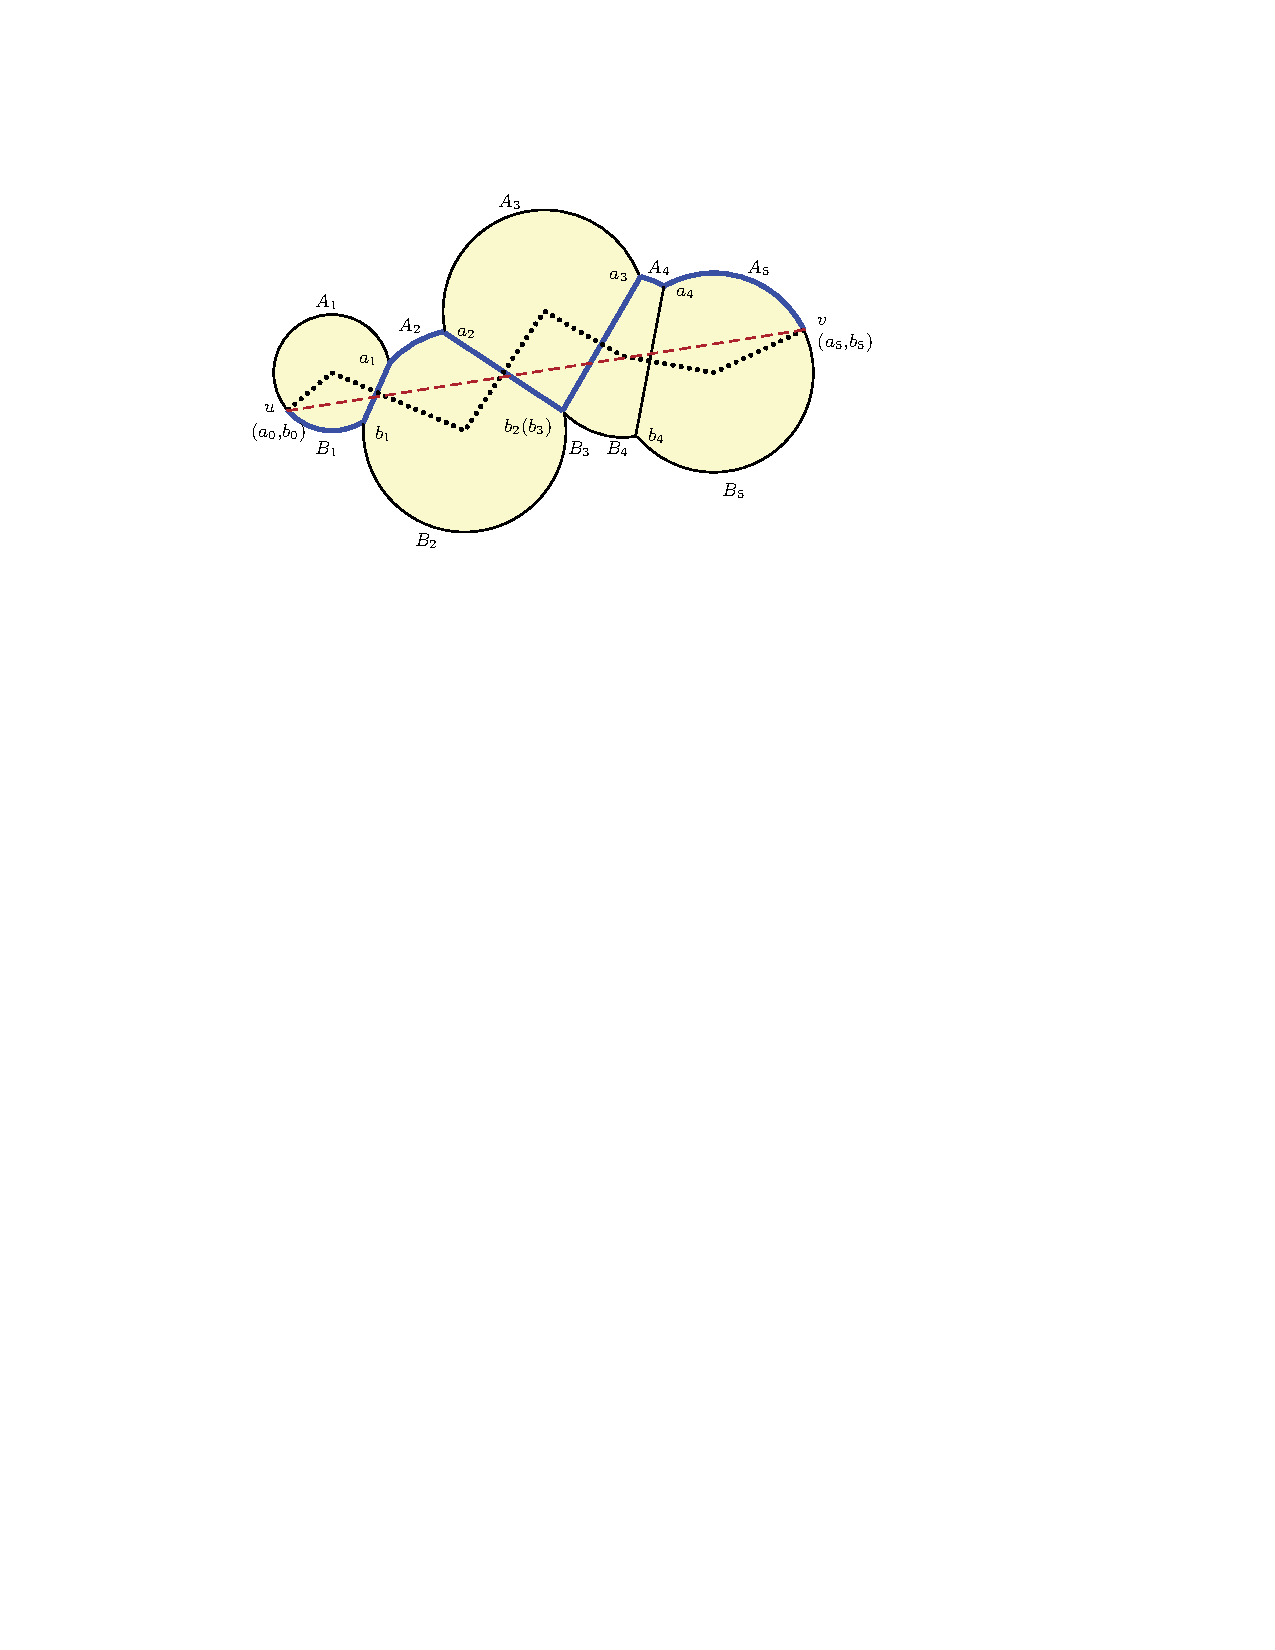
\includegraphics[width=.9\linewidth]{Figures/xia_a.pdf}
\caption{} \label{fig:xia_a}
\end{subfigure}
% \hspace*{\fill}

\begin{subfigure}{.8\textwidth}
\centering
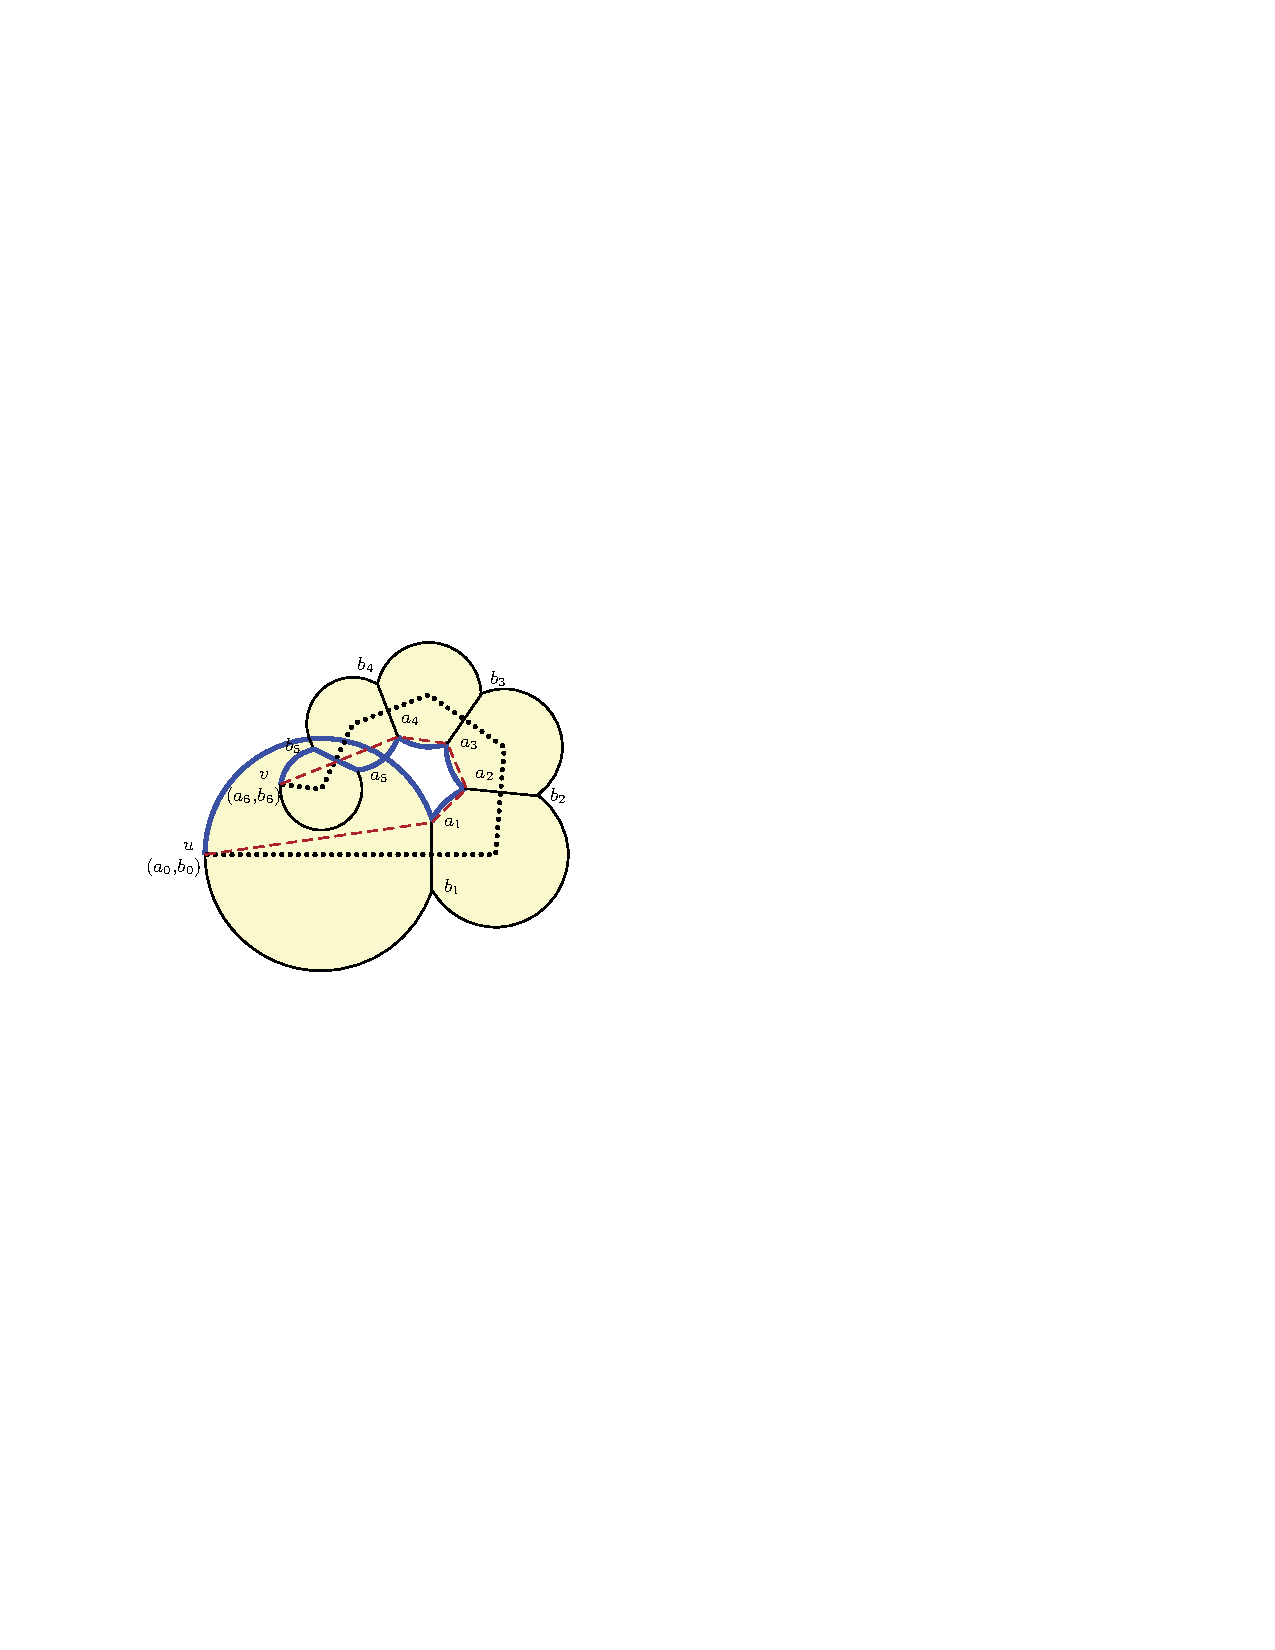
\includegraphics[width=.6\linewidth]{Figures/xia_b.pdf}
\caption{} \label{fig:xia_b}
\end{subfigure}
% \hspace*{\fill} % separation between the subfigures
\caption[Two illustrations of chains]{Two illustrations of chains. Terminal points $u$ and $v$ are unobstructed in Figure~\ref{fig:xia_a}. And Figure~\ref{fig:xia_b} shows the obstructed case.  Reprinted from \cite{xia}.} \label{fig:xia}
\end{figure}



\begin{definition}
Given a  chain $\mathcal{O} = \{O_1, O_2, \dots, O_n\}$. Choose points $u$ and $v$ on the boundary of $O_1$ and $O_n$  respectively. We say $u$ and $v$ are a pair of \textbf{terminal points} of $\mathcal{O}$. Denote the centers of $O_1, O_2, \dots, O_n$ as {$\boldsymbol{o_1, o_2, \dots, o_n}$} respectively. Then,  the \textbf{center polyline} between $u$ and $v$ is the polyline $uo_1\dots o_nv$. For $1\le i\le n-1$, let $\boldsymbol{a_i}$ and $\boldsymbol{b_i}$ be the intersections of the boundaries of $O_i$ and $O_{i+1}$. Without loss of generality, we say $a_i$'s are all on one side of the centered polyline, and $b_i$'s are on the other side. Also, define $\boldsymbol{a_0}=\boldsymbol{b_0} = u$ and $\boldsymbol{a_n}=\boldsymbol{b_n} = v$. For each disk $O_i$, denote the two arcs between the straight line segments $\overline{a_ib_i}$ and $\overline{a_{i-1}b_{i-1}}$ on the boundary of $O_i$ as $\boldsymbol{A_i}$ and $\boldsymbol{B_i}$, where $A_i$ has two end points $a_{i-1}$ and $a_i$ and $B_i$ has $b_{i-1}$ and $b_i$.
\end{definition}


\begin{definition}
Define $\boldsymbol{D_{\mathcal{O}}(u, v)}=up_1\dots p_{n-1}v$  as the shortest polyline from $u$ to $v$ that consists of line segments $\overline{up1}, \overline{p1p2}$, \dots, $\overline{p_{n-1}v}$ where $p_i\in\overline{a_ib_i}$ for $1\le i\le n-1$. That is, $D_{\mathcal{O}}(u, v)$
is the shortest polyline from $u$ to $v$ that intersects line segments $\overline{a_1b_1},\dots,\overline{a_{n-1}b_{n-1}}$ in order. Also, $\boldsymbol{|D_{\mathcal{O}}(u, v)|}$, the length of $D_{\mathcal{O}}(u, v)$, is the sum of lengths of all line segments in $D_{\mathcal{O}}(u, v)$.  
We say $u$ and $v$ are \textbf{obstructed} if the polyline $D_{\mathcal{O}}(u, v)$ contains a point $p_j$ which is either $a_j$ or $b_j$ for some $1\le j\le n-1$.
\end{definition}


\begin{proposition}
If $u$ and $v$ are not unobstructed, $ D_{\mathcal{O}}(u, v)$ is a straight line. 
\end{proposition}

\section{From Chains to Arcgons}
\begin{proposition}
Chains with unobstructed terminal points are equivalent to arcgons. 
\end{proposition}

\begin{proof}
We prove  the proposition by first expressing chains in graphs and then showing the expression in graph is equivalent to arcgons.

Let $\mathcal{O} = \{O_1, O_2, \dots, O_n\}$ be an  arbitrary chain. Suppose our terminal points $u$ and  $v$ are obstructed. Then, construct a graph $G$ whose edges are $\{A_1, A_2, \dots, A_n\}\cup \{B_1, B_2, \dots, B_n\} \cup \{\overline{a_1b_1},\overline{a_2b_2}, \dots \overline{a_{n-1}b_{n-1}} \}$, and vertices are $\{a_0, a_1, a_2, \dots, a_n\}\cup \{b_0, b_1, b_2, \dots, b_n\}$. Then, for all $1\le i\le n$, let $f_i$ be a graph constructed with $A_i, B_i, \overline{a_{i-1}a_i}$ and $\overline{b_{i-1}b_i}$. It is clear that $f_i$ is a face with a base circle $O_i$, and $F=\{f_1, f_2, \dots, f_n\}$ is a valid arcgon. Therefore, chains with unobstructed terminal points are equivalent to arcgons. 

On the other hand, suppose an arcgon $F=\{f_1, f_2, \dots, f_n\}$ is given. Let $\mathcal{C} = \{C_1, C_2, \dots, C_n\}$ be the base circles of $F$. Consider the disk bounded by each circle. Denote them as $\{O_1, O_2, \dots, O_n\}.$ Then, we can show that $\mathcal{O} = \{O_1, O_2, \dots, O_n\}$ is a chain with unobstructed terminal points. We know very two consecutive disks intersect because every consecutive faces share a diagonal in $F$. Also, since the arcgon $F$ is planar graph, the neighboring disks of every disk do not overlap. Therefore, all arcgons are chains with unobstructed terminal points.

We have shown the proposition.
\end{proof}


% \section{More on Arcgons}





% [Arcgon with condition 6 == chain with unobstructed terminal points]




% \begin{enumerate}
%     \item arcgon: modify there or explain more here about the p, q. The p, q is the same as p, q in chains. That is, any points on two end arcs are valid. but not for critical arcgons with complexity. of 1 b/c for paths over and below and one passing at least one diagonal, they must have the equal length. Thus, critical arcgons means fixed p and q.
    
%     \item define complexity.
    
%     Every stretch factor at most 
% \end{enumerate}


% arcgon

\chapter{Formulas}
\section{Complexity = 3}

We start from the case that complexity is $3$. 

Let a symmetric critical arcgon $\mathcal{F_3}$ be given. Let the base circles of $\mathcal{F}_3$ be $O_c', O_o$ and $O_c$. Since we will calculate the ratio between paths and absolute distance, the exact size of each circle does not matter. Without loss of generality, suppose that the muddle base circle, $O_o$, is a unite circle. That is, $o = (0, 0)$ and the radius of $O_o$ is $1$. Figure~\ref{fig:f1_1}(a) shows how we denote points in $\mathcal{F}_3$. 

\begin{figure}[ht]

\psset{unit=.7pt}
\psset{labelsep=7pt}
\begin{center} \small
\begin{pspicture}(-140,-150)(140,150)
    \psline{->}(-130,0)(130,0)
    \psline{->}(0, -130)(0, 130)
    \pscircle(0,0){100}
     \uput[45](0, 0){$o$}
     \psdot(0, 100)
      \uput[135](0, 100){$n$}
       \psdot(0, -100)
     \uput[-135](0, -100){$s$}
     \psdot(100, 0)
      \uput[225](100, 0){$e$}
      \psdot(-100, 0)
     \uput[-45](-100, 0){$w$}
     
    \psarc[linecolor=lightgray, linewidth=2pt](0,0){100}{-90}{8}
    % diagonal
    \psdot(99.268, 13.917)
    \uput[45](99.268, 13.917){$a$}
    \psline(0, -100)(99.268, 13.917)
    % center -> side circle
    \psdot(31.154, -27.082)
    \uput[90](31.154, -27.082){$c$}
    \pscircle(31.154, -27.082){79.27}
    \psarc[linecolor=lightgray, linewidth=2pt](31.154, -27.082){79.27}{31}{246.8}
    
     \psdot(49.343, -43.318)
     \uput[-45](49.343, -43.318){$m$}
     \psline[linestyle=dashed](31.154, -27.082)(49.343, -43.318)%cm
     
     \psdot(109.404, -14.408)
      \uput[0](109.404, -14.408){$q$}
    
    
    \psarc[linecolor=lightgray, linewidth=2pt](0,0){100}{172}{-90}
    % diagonal
    \psdot(-99.268, 13.917)
    \uput[135](-99.268, 13.917){$a'$}
    \psline(0, -100)(-99.268, 13.917)
    % center -> side circle
    \psdot(-31.154, -27.082)
    \uput[90](-31.154, -27.082){$c'$}
    \pscircle(-31.154, -27.082){79.27}
    \psarc[linecolor=lightgray, linewidth=2pt](-31.154, -27.082){79.27}{-66.8}{149}
     \psdot(-49.343, -43.318)
     \uput[225](-49.343, -43.318){$m'$}
     \psline[linestyle=dashed](-31.154, -27.082)(-49.343, -43.318)%cm
     \psdot(-109.404, -14.408)
      \uput[180](-109.404, -14.408){$p$}
    
    \psline[linecolor=red, linestyle= dashed](-109.404, -14.408)(109.404, -14.408)
    
    \uput[-90](0,-120){(a)}
\end{pspicture}
\psset{unit=.7pt}
\begin{pspicture}(-140,-150)(140,150)
    \psline{->}(-130,0)(130,0)
    \psline{->}(0, -130)(0, 130)
    \pscircle(0,0){100}
    %  \uput[45](0, 0){$o$}
    %  \psdot(0, 100)
    %   \uput[135](0, 100){$n$}
     \psdot(0, -100)
     \uput[-135](0, -100){$s$}
    %  \psdot(100, 0)
    %   \uput[225](100, 0){$e$}
    %   \psdot(-100, 0)
    %  \uput[-45](-100, 0){$w$}
     \uput[45](0, 100){$O_{up}$}
 
    \psarc[linecolor=lightgray, linewidth=2pt](0,0){100}{-90}{8}
    % diagonal
    \psdot(99.268, 13.917)
    \uput[45](99.268, 13.917){$a$}
    
    \psline(0, -100)(99.268, 13.917)
    % center -> side circle
    % \psdot(31.154, -27.082)
    % \uput[90](31.154, -27.082){$c$}
    \pscircle(31.154, -27.082){79.27}
    \psarc[linecolor=lightgray, linewidth=2pt](31.154, -27.082){79.27}{31}{246.8}
    
    %  \psdot(49.343, -43.318)
      \uput[-45](49.343, -43.318){$D$}
      \uput[225](98.646, -86.636){$B$}
    %  \psline[linestyle=dashed](31.154, -27.082)(49.343, -43.318)%cm
     
     \psdot(109.404, -14.408)
      \uput[0](109.404, -14.408){$q$}
       \uput[45](104.336,-0.2455){$A$}%a q mid point
    
    
    \psarc[linecolor=lightgray, linewidth=2pt](0,0){100}{172}{-90}
    % diagonal
    \psdot(-99.268, 13.917)
    \uput[135](-99.268, 13.917){$a'$}
    \psline(0, -100)(-99.268, 13.917)
    % center -> side circle
    % \psdot(-31.154, -27.082)
    % \uput[90](-31.154, -27.082){$c'$}
    \pscircle(-31.154, -27.082){79.27}
    \psarc[linecolor=lightgray, linewidth=2pt](-31.154, -27.082){79.27}{-66.8}{149}
    %  \psdot(-49.343, -43.318)
     \uput[225](-49.343, -43.318){$D'$}
     \uput[-45 ](-98.646, -86.636){$B'$}
    %  \psline[linestyle=dashed](-31.154, -27.082)(-49.343, -43.318)%cm
     \psdot(-109.404, -14.408)
      \uput[180](-109.404, -14.408){$p$}
       \uput[135](-104.336,-0.2455){$A'$}%a q mid point
    
    
    % \psline[linecolor=red, linestyle= dashed](-109.404, -14.408)(109.404, -14.408)
 \uput[-90](0,-120){(b)}
\end{pspicture}

\caption[Illustrations on denotions.]{Illustrations on denotions.
(a) The centers of three circles are denoted as $c'$, $o$ and $c$ respectively. The intersect between $O_o$ with axis are $n, s, w$ and $e$. $O_c'$ and $O_o$ intersect at $a'$, and $O_c$ and $O_o$ intersect at $a$. Let $p, q$ be terminal points of $\mathcal{F}_3$.And let $m, m'$ be the midpoints of $as$ and $a's$ respectively.
(b) Let $\overline{a's}, \overline{as}$ be diagonals $D'$ and $D$. Arcs are defined as the following: $A' = \arc{pa'}$, $A = \arc{pa}$, $B' = \arc{ps}$, $B = \arc{qs}$, $O_{up} = \arc{a'na}$.
}\label{fig:f1_1}
\end{center}
\end{figure} 



Figure~\ref{fig:f1_1}(b) gives an illustration on arcs. Since $\mathcal{F}_3$ is symmetric, we know that 
\[A' = A\text{, } B'= B\text{, }D' = D \text{, }\arc{a'n} = \arc{na}.\]
Also, paths from $p$ to $q$ in $\mathcal{F}_3$ could be
\[A'O_{up}A\text{, }A'D'DA\text{, } A'D'B\text{, }B'DA\text{, } B'B.\]
Since $\mathcal{F}_3$ is critical, all paths listed above have the same length.
Let $\|\overline{sm}| = |\overline{am}| = x$ and $|\overline{cm}| = k$. 
\begin{theorem}
$\rho_{\mathcal{F}_3}(p, q) =  \cfrac{x + \sqrt{k^2+x^2}\cdot\tan^{-1}{\frac{x}{k}}}{\left(\sqrt{1- x^2} - k\right)\cdot\cos{x} + \sqrt{k^2 + x^2}\cdot\cos{\left(\frac{x}{\sqrt{k^2 + x^2}} - x\right)}}.$
\end{theorem}

\begin{proof}

[Goal 1: Find a solution of $x$.]


Let $r$ be the radius of $O_c$ and $O_c'$. That is, $r = \sqrt{x^2+k^2}$.

First, we can show that $\arc{na} = 2x$. Since $A'O_{up}A$ and 
$A'D'DA$ are equal in length, we have
\begin{align*}
    |O_{up}| &= |D'D| \\
    |\arc{a'n}|+|\arc{na}| &= |D'|+|D|.
\end{align*}
Also, since $|\arc{a'n}|=|\arc{na}|$ and $|D'|=|D|$, then
\begin{align*}
    2|\arc{na}| &= 2|D|, \\
    |\arc{na}|&= |D| \\
    &=|\overline{am}|+|\overline{ms}|\\
    &=x+x\\
    &=2x.
\end{align*}

Consider $\arc{aws}$. Since $|\overline{am}| = x$ and  $|\overline{oa}| = 1$, we know $\angle aom = \sin^{-1}{x}$.
Thus,
\begin{align*}
    \arc{aws} &= 2 (1\cdot\angle aom)= 2\cdot \sin^{-1}{x}.
\end{align*}
Then, since $\arc{an}$ and $\arc{aws}$ construct a semicircle, we have
\begin{align*}
    |\arc{\overline{an}}+\arc{aws}| &= \pi \\
    2x +2\sin^{-1}{x} &= \pi\\
    x +\sin^{-1}{x} - \frac{\pi}{2} & = 0.\\
\end{align*}
Therefore,  $x$ is the solution of $x +\sin^{-1}{x} - \frac{\pi}{2}= 0$. The approximate value is $0.739085$.



\vspace{1cm}
[Goal 2: Calculate $P_{\mathcal{F}_3}(p, q)$.]
\begin{figure}[ht]

\psset{unit=.7pt}
\psset{labelsep=7pt}
\begin{center} \small
\begin{pspicture}(-140,-150)(140,150)
    \psline{->}(-130,0)(130,0)
    \psline{->}(0, -130)(0, 130)
    \pscircle(0,0){100}
     \uput[45](0, 0){$o$}
     \psdot(0, 100)
      \uput[135](0, 100){$n$}
       \psdot(0, -100)
     \uput[-135](0, -100){$s$}
     \psdot(100, 0)
      \uput[225](100, 0){$e$}
      \psdot(-100, 0)
     \uput[-45](-100, 0){$w$}
     
    \psarc[linecolor=lightgray, linewidth=2pt](0,0){100}{-90}{8}
    % diagonal
    \psdot(99.268, 13.917)
    \uput[45](99.268, 13.917){$a$}
    \psline(0, -100)(99.268, 13.917)
    % center -> side circle
    \psdot(31.154, -27.082)
    \uput[90](31.154, -27.082){$c$}
    \pscircle(31.154, -27.082){79.27}
    \psarc[linecolor=lightgray, linewidth=2pt](31.154, -27.082){79.27}{31}{246.8}
    
    \psline[linestyle=dashed](0, 0)(99.268, 13.917)%oa
    \psline[linestyle=dashed](31.154, -27.082)(99.268, 13.917)%ca
    \psline[linestyle=dashed](0, 0)(31.154, -27.082)%oc
    
    
     \psdot(49.343, -43.318)
     \uput[-45](49.343, -43.318){$m$}
     \psline[linestyle=dashed](31.154, -27.082)(49.343, -43.318)%cm
     
     \psdot(109.404, -14.408)
      \uput[0](109.404, -14.408){$q$}
    
    
    \psarc[linecolor=lightgray, linewidth=2pt](0,0){100}{172}{-90}
    % diagonal
    % \psdot(-99.268, 13.917)
    % \uput[135](-99.268, 13.917){$a'$}
    \psline(0, -100)(-99.268, 13.917)
    % center -> side circle
    % \psdot(-31.154, -27.082)
    % \uput[90](-31.154, -27.082){$c'$}
    \pscircle(-31.154, -27.082){79.27}
    \psarc[linecolor=lightgray, linewidth=2pt](-31.154, -27.082){79.27}{-66.8}{149}
    %  \psdot(-49.343, -43.318)
    %  \uput[225](-49.343, -43.318){$m'$}
    %  \psline[linestyle=dashed](-31.154, -27.082)(-49.343, -43.318)%cm
     \psdot(-109.404, -14.408)
      \uput[180](-109.404, -14.408){$p$}
    
    % \psline[linecolor=red, linestyle= dashed](-109.404, -14.408)(109.404, -14.408)
    
    \uput[-90](0,-120){(a)}
\end{pspicture}
\psset{unit=.7pt}
\begin{pspicture}(-140,-150)(140,150)
    \psline{->}(-130,0)(130,0)
    \psline{->}(0, -130)(0, 130)
    \pscircle(0,0){100}
     \uput[45](0, 0){$o$}
     \psdot(0, 100)
      \uput[135](0, 100){$n$}
       \psdot(0, -100)
     \uput[-135](0, -100){$s$}
     \psdot(100, 0)
      \uput[225](100, 0){$e$}
      \psdot(-100, 0)
     \uput[-45](-100, 0){$w$}
     
    \psarc[linecolor=lightgray, linewidth=2pt](0,0){100}{-90}{8}
    % diagonal
    \psdot(99.268, 13.917)
    \uput[45](99.268, 13.917){$a$}
    
    
    \psline(0, -100)(99.268, 13.917)
    % center -> side circle
    \psdot(31.154, -27.082)
    \uput[90](31.154, -27.082){$c$}
    \pscircle(31.154, -27.082){79.27}
    \psarc[linecolor=lightgray, linewidth=2pt](31.154, -27.082){79.27}{31}{246.8}
    
    \psline[linestyle=dashed](0, 0)(99.268, 13.917)%oa
    \psline[linestyle=dashed](31.154, -27.082)(99.268, 13.917)%ca
    \psline[linestyle=dashed](0, 0)(31.154, -27.082)%oc
    
    
     \psdot(49.343, -43.318)
     \uput[-45](49.343, -43.318){$m$}
     \psline[linestyle=dashed](31.154, -27.082)(49.343, -43.318)%cm
     
     \psdot(109.404, -14.408)
      \uput[0](109.404, -14.408){$q$}
    
    
    % \psarc[linecolor=lightgray, linewidth=2pt](0,0){100}{172}{-90}
    % diagonal
    % \psdot(-99.268, 13.917)
    % \uput[135](-99.268, 13.917){$a'$}
    % \psline(0, -100)(-99.268, 13.917)
    % center -> side circle
    % \psdot(-31.154, -27.082)
    % \uput[90](-31.154, -27.082){$c'$}
    % \pscircle(-31.154, -27.082){79.27}
    % \psarc[linecolor=lightgray, linewidth=2pt](-31.154, -27.082){79.27}{-66.8}{149}
    %  \psdot(-49.343, -43.318)
    %  \uput[225](-49.343, -43.318){$m'$}
    %  \psline[linestyle=dashed](-31.154, -27.082)(-49.343, -43.318)%cm
    %  \psdot(-109.404, -14.408)
      \uput[180](-109.404, -14.408){$p$}
    % 
    % \psline[linecolor=red, linestyle= dashed](-109.404, -14.408)(109.404, -14.408)
    
    \uput[45](71, 71){$2x$}
    \uput[-45](103, -103){$2r\cdot \tan^{-1}\frac{x}{k}$}
    
    \uput[-90](0,-120){(b)}
\end{pspicture}

\caption[Calculate the path distance from $p$ to $q$. ]{Calculate the path distance from $p$ to $q$.}\label{fig:f1_2}
\end{center}
\end{figure} 


According to Figure~\ref{fig:f1_2}, %??????f1-2
$A'O_{up}A$ and $B'B$ are two path from $p$ to $q$. Then, we have
\begin{align*}
    2 P_{\mathcal{F}_3}(p, q) & = |A'O_{up}A|+|B'B|\\
    P_{\mathcal{F}_3}(p, q) & = \frac{|A'O_{up}A|}{2}+\frac{|B'B|}{2}\\
    &= |\arc{na}|+|A|+|B|\\
    &=|\arc{na}|+|\arc{aqs}|.
\end{align*}
We have shown that $|\arc{na}| = 2x$. Also, we know that $|\arc{aqs}| = 2(r\cdot \angle acm)$, and $\angle acm = \tan^{-1}{\frac{x}{k}}$. Thus,
\[|\arc{aqs}| = 2r\cdot \tan^{-1}{\frac{x}{k}}.\]
Therefore, 
\begin{align*}
    P_{\mathcal{F}_3}(p, q) &=|\arc{na}|+|\arc{aqs}|\\
    &=2x + 2r\cdot \tan^{-1}{\frac{x}{k}}.
\end{align*}


\vspace{1cm}
[Goal 3: Calculate $D_{\mathcal{F}_3}(p, q)$.]
\begin{figure}[ht]

\psset{unit=.7pt}
\psset{labelsep=7pt}
% \begin{center} \small
\begin{pspicture}(-140,-150)(140,150)
    \psline{->}(-130,0)(130,0)
    \psline{->}(0, -130)(0, 130)
    \pscircle(0,0){100}
     \uput[45](0, 0){$o$}
     \psdot(0, 100)
      \uput[135](0, 100){$n$}
       \psdot(0, -100)
     \uput[-135](0, -100){$s$}
     \psdot(100, 0)
      \uput[225](100, 0){$e$}
      \psdot(-100, 0)
     \uput[-45](-100, 0){$w$}
     
    \psarc[linecolor=lightgray, linewidth=2pt](0,0){100}{-90}{8}
    % diagonal
    \psdot(99.268, 13.917)
    \uput[45](99.268, 13.917){$a$}
    \psline(0, -100)(99.268, 13.917)
    % center -> side circle
    \psdot(31.154, -27.082)
    \uput[90](31.154, -27.082){$c$}
    \pscircle(31.154, -27.082){79.27}
    \psarc[linecolor=lightgray, linewidth=2pt](31.154, -27.082){79.27}{31}{246.8}
    
     \psdot(49.343, -43.318)
     \uput[-45](49.343, -43.318){$m$}
     \psline[linestyle=dashed](31.154, -27.082)(49.343, -43.318)%cm
     
     \psdot(109.404, -14.408)
      \uput[0](109.404, -14.408){$q$}
    
    
    \psarc[linecolor=lightgray, linewidth=2pt](0,0){100}{172}{-90}
    % diagonal
    \psdot(-99.268, 13.917)
    \uput[135](-99.268, 13.917){$a'$}
    \psline(0, -100)(-99.268, 13.917)
    % center -> side circle
    \psdot(-31.154, -27.082)
    \uput[90](-31.154, -27.082){$c'$}
    \pscircle(-31.154, -27.082){79.27}
    \psarc[linecolor=lightgray, linewidth=2pt](-31.154, -27.082){79.27}{-66.8}{149}
     \psdot(-49.343, -43.318)
     \uput[225](-49.343, -43.318){$m'$}
     \psline[linestyle=dashed](-31.154, -27.082)(-49.343, -43.318)%cm
     \psdot(-109.404, -14.408)
      \uput[180](-109.404, -14.408){$p$}
    
    \psline[linecolor=red, linestyle= dashed](-109.404, -14.408)(109.404, -14.408)
    
    \uput[-90](0,-120){(a) . }
\end{pspicture}
\psset{unit=.7pt}
\begin{pspicture}(-140,-150)(140,150)
    \psline{->}(-130,0)(130,0)
    \psline{->}(0, -130)(0, 130)
    \pscircle(0,0){100}
    %  \uput[45](0, 0){$o$}
    %  \psdot(0, 100)
    %   \uput[135](0, 100){$n$}
     \psdot(0, -100)
     \uput[-135](0, -100){$s$}
    %  \psdot(100, 0)
    %   \uput[225](100, 0){$e$}
    %   \psdot(-100, 0)
    %  \uput[-45](-100, 0){$w$}
     \uput[45](0, 100){$O_{up}$}
 
    \psarc[linecolor=lightgray, linewidth=2pt](0,0){100}{-90}{8}
    % diagonal
    \psdot(99.268, 13.917)
    \uput[45](99.268, 13.917){$a$}
    
    \psline(0, -100)(99.268, 13.917)
    % center -> side circle
    % \psdot(31.154, -27.082)
    % \uput[90](31.154, -27.082){$c$}
    \pscircle(31.154, -27.082){79.27}
    \psarc[linecolor=lightgray, linewidth=2pt](31.154, -27.082){79.27}{31}{246.8}
    
    %  \psdot(49.343, -43.318)
      \uput[-45](49.343, -43.318){$D$}
      \uput[225](98.646, -86.636){$B$}
    %  \psline[linestyle=dashed](31.154, -27.082)(49.343, -43.318)%cm
     
     \psdot(109.404, -14.408)
      \uput[0](109.404, -14.408){$q$}
       \uput[45](104.336,-0.2455){$A$}%a q mid point
    
    
    \psarc[linecolor=lightgray, linewidth=2pt](0,0){100}{172}{-90}
    % diagonal
    \psdot(-99.268, 13.917)
    \uput[135](-99.268, 13.917){$a'$}
    \psline(0, -100)(-99.268, 13.917)
    % center -> side circle
    % \psdot(-31.154, -27.082)
    % \uput[90](-31.154, -27.082){$c'$}
    \pscircle(-31.154, -27.082){79.27}
    \psarc[linecolor=lightgray, linewidth=2pt](-31.154, -27.082){79.27}{-66.8}{149}
    %  \psdot(-49.343, -43.318)
     \uput[225](-49.343, -43.318){$D'$}
     \uput[-45 ](-98.646, -86.636){$B'$}
    %  \psline[linestyle=dashed](-31.154, -27.082)(-49.343, -43.318)%cm
     \psdot(-109.404, -14.408)
      \uput[180](-109.404, -14.408){$p$}
       \uput[135](-104.336,-0.2455){$A'$}%a q mid point
    
    
    % \psline[linecolor=red, linestyle= dashed](-109.404, -14.408)(109.404, -14.408)
 \uput[-90](0,-120){(b) Example 2. }
\end{pspicture}

\caption{
}\label{fig:f1_3}
% \end{center}
\end{figure} 


Let $\overline{oc_x}$ and $\overline{cq_x}$ be the images of $\overline{oc}$ and $\overline{cq}$ in positive $x$ direction respectively. Then, we have
\[\frac{D_{\mathcal{F}_3}(p, q)}{2} = |oc_x|+|cq_x|.\]

Consider $|\overline{oc_x}|$. Since $|\overline{xs}| = x$, we have $\angle soc = \sin^{-1}{x}$. Then,
\begin{align*}
    \angle c_xoc &=\angle c_xos + \angle soc\\
    &=-\frac{\pi}{2}+\sin^{-1}x.
\end{align*}
Since we have shown that $x+\sin^{-1}x-\frac{\pi}{2} = 0$, we know
\[\angle c_xoc = -x.\]
Then, since $|\overline{om}| = \sqrt{|\overline{oa}|^2-|\overline{am}|^2} = \sqrt{1-x^2}$, and we defined $|\overline{cm}| = k$, 
\begin{align*}
    |\overline{oc}| &= |\overline{om}|-|\overline{cm}|\\
    &= \sqrt{1-x^2} - k.
\end{align*}
Therefore, 
\begin{align*}
    |\overline{oc_x}| &= |\overline{oc}|\cdot\angle c_xoc\\
    &= (\sqrt{1-x^2} - k)\cdot \cos{(-x)}.
\end{align*}

Consider $|\overline{
cq_x}|$. The angle from positive $x$ direction to $cq$ is
\[\angle q_xcq = \angle q_xcm+\angle mca - \angle qca.\]


\begin{figure}[ht]

\psset{unit=.7pt}
\psset{labelsep=7pt}
% \begin{center} \small
\begin{pspicture}(-140,-150)(140,150)
    \psline{->}(-130,0)(130,0)
    \psline{->}(0, -130)(0, 130)
    \pscircle(0,0){100}
     \uput[45](0, 0){$o$}
     \psdot(0, 100)
      \uput[135](0, 100){$n$}
       \psdot(0, -100)
     \uput[-135](0, -100){$s$}
     \psdot(100, 0)
      \uput[225](100, 0){$e$}
      \psdot(-100, 0)
     \uput[-45](-100, 0){$w$}
     
    \psarc[linecolor=lightgray, linewidth=2pt](0,0){100}{-90}{8}
    % diagonal
    \psdot(99.268, 13.917)
    \uput[45](99.268, 13.917){$a$}
    \psline(0, -100)(99.268, 13.917)
    % center -> side circle
    \psdot(31.154, -27.082)
    \uput[90](31.154, -27.082){$c$}
    \pscircle(31.154, -27.082){79.27}
    \psarc[linecolor=lightgray, linewidth=2pt](31.154, -27.082){79.27}{31}{246.8}
    
     \psdot(49.343, -43.318)
     \uput[-45](49.343, -43.318){$m$}
     \psline[linestyle=dashed](31.154, -27.082)(49.343, -43.318)%cm
     
     \psdot(109.404, -14.408)
      \uput[0](109.404, -14.408){$q$}
    
    
    \psarc[linecolor=lightgray, linewidth=2pt](0,0){100}{172}{-90}
    % diagonal
    \psdot(-99.268, 13.917)
    \uput[135](-99.268, 13.917){$a'$}
    \psline(0, -100)(-99.268, 13.917)
    % center -> side circle
    \psdot(-31.154, -27.082)
    \uput[90](-31.154, -27.082){$c'$}
    \pscircle(-31.154, -27.082){79.27}
    \psarc[linecolor=lightgray, linewidth=2pt](-31.154, -27.082){79.27}{-66.8}{149}
     \psdot(-49.343, -43.318)
     \uput[225](-49.343, -43.318){$m'$}
     \psline[linestyle=dashed](-31.154, -27.082)(-49.343, -43.318)%cm
     \psdot(-109.404, -14.408)
      \uput[180](-109.404, -14.408){$p$}
    
    \psline[linecolor=red, linestyle= dashed](-109.404, -14.408)(109.404, -14.408)
    
    \uput[-90](0,-120){(a) . }
\end{pspicture}
\psset{unit=.7pt}
\begin{pspicture}(-140,-150)(140,150)
    \psline{->}(-130,0)(130,0)
    \psline{->}(0, -130)(0, 130)
    \pscircle(0,0){100}
    %  \uput[45](0, 0){$o$}
    %  \psdot(0, 100)
    %   \uput[135](0, 100){$n$}
     \psdot(0, -100)
     \uput[-135](0, -100){$s$}
    %  \psdot(100, 0)
    %   \uput[225](100, 0){$e$}
    %   \psdot(-100, 0)
    %  \uput[-45](-100, 0){$w$}
     \uput[45](0, 100){$O_{up}$}
 
    \psarc[linecolor=lightgray, linewidth=2pt](0,0){100}{-90}{8}
    % diagonal
    \psdot(99.268, 13.917)
    \uput[45](99.268, 13.917){$a$}
    
    \psline(0, -100)(99.268, 13.917)
    % center -> side circle
    % \psdot(31.154, -27.082)
    % \uput[90](31.154, -27.082){$c$}
    \pscircle(31.154, -27.082){79.27}
    \psarc[linecolor=lightgray, linewidth=2pt](31.154, -27.082){79.27}{31}{246.8}
    
    %  \psdot(49.343, -43.318)
      \uput[-45](49.343, -43.318){$D$}
      \uput[225](98.646, -86.636){$B$}
    %  \psline[linestyle=dashed](31.154, -27.082)(49.343, -43.318)%cm
     
     \psdot(109.404, -14.408)
      \uput[0](109.404, -14.408){$q$}
       \uput[45](104.336,-0.2455){$A$}%a q mid point
    
    
    \psarc[linecolor=lightgray, linewidth=2pt](0,0){100}{172}{-90}
    % diagonal
    \psdot(-99.268, 13.917)
    \uput[135](-99.268, 13.917){$a'$}
    \psline(0, -100)(-99.268, 13.917)
    % center -> side circle
    % \psdot(-31.154, -27.082)
    % \uput[90](-31.154, -27.082){$c'$}
    \pscircle(-31.154, -27.082){79.27}
    \psarc[linecolor=lightgray, linewidth=2pt](-31.154, -27.082){79.27}{-66.8}{149}
    %  \psdot(-49.343, -43.318)
     \uput[225](-49.343, -43.318){$D'$}
     \uput[-45 ](-98.646, -86.636){$B'$}
    %  \psline[linestyle=dashed](-31.154, -27.082)(-49.343, -43.318)%cm
     \psdot(-109.404, -14.408)
      \uput[180](-109.404, -14.408){$p$}
       \uput[135](-104.336,-0.2455){$A'$}%a q mid point
    
    
    % \psline[linecolor=red, linestyle= dashed](-109.404, -14.408)(109.404, -14.408)
 \uput[-90](0,-120){(b) Example 2. }
\end{pspicture}

\caption{
}\label{fig:f1_4}
% \end{center}
\end{figure} 

%?????????


We  have shown  that the angle from positive $x$ direction to $\overrightarrow{oc}$ is $-x$. Then, since $o, c$ and $m$ are co-linear, we say $\angle q_xcm = -x$ as well. Also, we know that $\angle mca = \tan^{-1}\frac{x}{k}$. 

We will calculate $\angle qca$ by analyzing arc $A$. Since $\mathcal{F}_3$ is  critical and symmetric, we have
\begin{align*}
    |A'D'DA| &=|B'B|\\
    |A|+|D| &= |B|\\
    |A| &= |B|-|D|.
\end{align*}
Then, given $|A|+|B| = |\arc{aqs}| = 2r\cdot \tan^{-1}\frac{x}{k}$ and $|D|=2|\overline{aw}| = 2x$, we have
\begin{align*}
    |A| &= |B| - |D|\\
    |A| &= |\arc{aqs}|-|A|  - |D|\\
    2|A| &= |\arc{aqs}|- |D|\\
    |A| &=\frac{|\arc{aqs}|- |D|}{2}\\
    &=\frac{2r\cdot \tan^{-1}\frac{x}{k} - 2x}{2}\\
    &=r\cdot \tan^{-1}\frac{x}{k} - x.
\end{align*}
Thus, $\angle qca = \frac{|A|}{r}$, and
\begin{align*}
    \angle q_xcq &= \angle q_xcm+\angle mca - \angle qca\\
    &= -x +\tan^{-1}\frac{x}{k}-\frac{r\cdot \tan^{-1}\frac{x}{k} - x}{r}\\
    &= -x +\tan^{-1}\frac{x}{k}-(\tan^{-1}\frac{x}{k} - \frac{x}{r})\\
    &=-x+\frac{x}{r}.
\end{align*}
Therefore, 
   \[|cq_x| = r\cdot \cos{(\angle q_xcq)}= r\cdot\cos{(-x+\frac{x}{r})}.\]
Then, 
\begin{align*}
    \frac{D_{\mathcal{F}_3}(p, q)}{2} &= |oc_x|+|cq_x|\\
    &=(\sqrt{1-x^2} - k)\cdot \cos{(-x)} +r\cdot \cos{(-x+\frac{x}{r})}.
\end{align*}
\vspace{1cm}
Hence, 
\begin{align*}
    \rho_{\mathcal{F}_3}(p, q) &=  \frac{P_{\mathcal{F}_3}(p, q)}{D_{\mathcal{F}_3}(p, q)}\\
    &=\frac{P_{\mathcal{F}_3}(p, q)/2}{D_{\mathcal{F}_3}(p, q)/2}\\
     &=\frac{\frac{2x+2r\cdot\tan^{-1}\frac{x}{k}}{2}}{(\sqrt{1-x^2} - k)\cdot \cos{(-x)} +r\cdot \cos{(-x+\frac{x}{r})}}\\
     &=\frac{x+r\cdot\tan^{-1}\frac{x}{k}}{(\sqrt{1-x^2} - k)\cdot \cos{(-x)} +r\cdot \cos{(-x+\frac{x}{r})}}\text{, as desired. }
\end{align*}
\end{proof}

\section{In the General Case}
	Consider the symmetric critical arcgons with $2n+1$ circles. Suppose the formula for $2(n-1)+1$ circles is given, the length for the shortest path should increment by $(\sqrt{r_N- x_N^2} - k_N)\cdot\cos(\tan^{-1}{\frac{x_j}{r_j}}-  \sin^{-1}{\frac{x_j}{k_j}}) $.

	For any symmetric critical arcgons with $2n + 1$ circles, 
	\[d(\vec{x}, \vec{k}) = \sum_{1\le i< n}\left(\sqrt{r_i- x_i^2} - k_i\right)\cdot\cos\left({x_1 +\sum_{1\le j< i} \tan^{-1}{\frac{x_j}{r_j}}-  \sin^{-1}{\frac{x_j}{k_j}}}\right) \]
	\[p(\vec{x}, \vec{k}) = x_1 + \sum_{1\le i< n}r_i\cdot(\tan^{-1}{\frac{x_i}{k_i}}- \sin^{-1}{\frac{x_{i+1}}{r_i}}) + r_n\tan^{-1}{\frac{x_n}{k_n}}.\]

\chapter{On the Lower Bound}
We proceed by showing the existence of a symmetric critical arcgon with stretch factor $1.59324$. 
The following is an algorithm to estimate the lower bound for the stretch factor of symmetric critical arcgon. 

\begin{algorithm}
\caption{Find the minmun value of function func}
\label{check}
\begin{algorithmic}[1]
\Procedure{Check}{$n$}
\State $func(\vec{x},\vec{k}) = d(\vec{x},\vec{k})/p(\vec{x},\vec{k})) $
\For{every $x$, $\vec{x'}$ and every $\vec{k'}$ }
\State temp = $func(\vec{x'}, \vec{k'})$
\If{temp $>$ max}
\State max = temp
\State Return $max$
\EndIf
\EndFor
\EndProcedure
\end{algorithmic}
\end{algorithm}



Applying the algorithm on varied $n$ and the corresponding formula gives the worst cases. The table below gives the worst case of the stretch factors with $5, 7, 9, 11$  and $13$ circles respectively.
\begin{table}[ht]
\centering
\begin{tabular}{l|l}
the Number of Circles & the Worst Case \\ \hline
5                     & 1.5932135      \\
7                     & 1.5932263      \\
9                     & 1.5932389      \\
11                    & 1.5932412      \\
13                    & 1.5932413     
\end{tabular}
\end{table}

\vspace{1in}

\chapter{On the Upper Bound}
Consider a Let $\mathcal{O}$ be a chain of three distinct disks where $\mathcal{O} = (O_1, O_2, O_3)$. Define $D_\mathcal{O}(u,v)$ to be the shortest polyline from $u$ to $v$ 
% that intersects line segments $a_1b_1, \dots , a_{n−1}b_{n−1}$ in that order
and $P_\mathcal{O}(u,v)$ to be the shortest path from $u$ to $v$
% that consists of arcs in {A1,...,An}∪ {B1, . . . , Bn} and line segments in {a1b1, . . . , an−1bn−1}.
.
Then, let $d(x, k) = \left|D_\mathcal{O}(u,v)\right|$ and $p(x, k) =| P_\mathcal{O}(u,v) |$ where $x$ is $\frac{|\overline{AB}|}{2}$ and $k$ is the distance from $O_3$ to the string $\overline{AB}$.
Thus, we have
\[d(x, k) = \left(\sqrt{1- x^2} - k\right)\cdot\cos{x} + \sqrt{k^2 + x^2}\cdot\cos{\left(\frac{x}{\sqrt{k^2 + x^2}} - x\right)},\]
\[p(x, k) = \frac{\pi}{2} - \sin^{-1}{x} + \sqrt{k^2+x^2}\cdot\tan^{-1}{\frac{x}{k}}.\]

Note that $x\in (0, 0.739)$, and $k\in (0, \sqrt{1-x^2})$ for a given $x$. 

\begin{theorem}
For all $0<x<0.739$ and $0<k<\sqrt{1-x^2}$, $\frac{p(x, k)}{d(x, k)} < 1.6$.
\end{theorem}
Let $x\in (0, 0.739)$ be given. Choose a $k$ such that $0< k < \sqrt{1-x^2}$. Let $r = \sqrt{k^2 + x^2}$.
Define 
\[f(x, k, \sigma) = p(x, k) - \sigma\cdot d(x, k).\] 

[Goal: Show that $f(x, k, \sigma) < 0$ when $\sigma = 1.6$.]

Calculating the partial derivatives for $f$ and replacing $\sqrt{k^2 + x^2}$ by $r$ give
\begin{align*}
    \frac{\partial f}{\partial x}  = &\frac{-1+x\cdot\sigma\cdot\cos{x}}{\sqrt{1-x^2}} 
+ \frac{k+ x\cdot\tan^{-1}{(\frac{x}{k})}+ x\cdot\sigma\cdot\cos{(x-\frac{x}{r})}}{r}\\
&+ \frac{(-k^2+ r^3)\cdot\sigma\sin{(x-\frac{x}{r})}}{r^2}
+ (\sqrt{1-x^2}-k)\cdot \sigma\cdot\sin{x} ,
\end{align*}
and
\begin{align*}
    \frac{\partial f}{\partial k}  = & -\frac{x}{r} 
    + \sigma\cdot\cos x
    + \frac{k(r\cdot \tan^{-1}(\frac{x}{k})- r\cdot\sigma\cos(x-\frac{x}{r}) + x\sigma\cdot \sin^{-1}(x-\frac{x}{r}))}{r^2}.
\end{align*}
Note that $k, x < \sqrt{k^2 + x^2} = r$, and for all $\alpha\in \mathbb{R}$ $\cos\alpha, \sin\alpha < 1$ and $\tan^{-1}\alpha, \sin^{-1}\alpha <\frac{\pi}{2}$. 

Then, for  $\frac{-1+x\cdot\sigma\cdot\cos{x}}{\sqrt{1-x^2}}$, if $x\le\sqrt{1-x^2}$, we have 
\begin{align*} 
\frac{-1+x\cdot\sigma\cdot\cos{x}}{\sqrt{1-x^2}}
&  < \frac{x}{\sqrt{1-x^2}}\cdot\sigma\cdot\cos{x}\\
& < \sigma
\end{align*}
If  $x>\sqrt{1-x^2}$, let $g(x) = x\cdot\cos x - \sqrt{1-x^2}.$ Then, $g'(x) = \frac{x}{\sqrt{1-x^2}} + \cos x - x\cdot \sin x$. Since $x > \sqrt{1 - x^2}$, $\frac{x}{\sqrt{1-x^2}}> 1$. Thus,
\begin{align*} 
g'(x) & >  \frac{x}{\sqrt{1-x^2}} - x\cdot \sin x\\
& > 1-- x\cdot \sin x\\
& > 0.
\end{align*}
Therefore, since $x < 1$, $g(x) < g(1) = \cos 1$.
Then, 
\begin{align*} 
x\cdot\cos x - \sqrt{1-x^2} & < \cos 1\\
x\cdot\cos x - \sqrt{1-x^2} & < \frac{1}{\sigma}\\
\frac{-1+x\cdot\sigma\cdot\cos{x}}{\sqrt{1-x^2}}  & < \sigma.
\end{align*}
Therefore, 
\begin{align} \label{part1}
\frac{-1+x\cdot\sigma\cdot\cos{x}}{\sqrt{1-x^2}} &  < \sigma
\end{align}
\begin{align}\label{part2}
\frac{k+ x\cdot\tan^{-1}{(\frac{x}{k})}+ x\cdot\sigma\cdot\cos{(x-\frac{x}{r})}}{r}
&  = \frac{k}{r} + \frac{x}{r}\cdot\tan^{-1}{(\frac{x}{k})} + \frac{x}{r}\cdot\sigma\cdot\cos(x-\frac{x}{r})\nonumber\\
& < 1 + \frac{\pi}{2} 
\end{align}
\begin{align}\label{part3}
\frac{(-k^2+ r^3)\cdot\sigma\sin{(x-\frac{x}{r})}}{r^2} & < \frac{ r^3}{r^2}\cdot\sigma\sin{(x-\frac{x}{r})}\nonumber\\
& < \sigma.
\end{align}
\begin{align}\label{part4}
(\sqrt{1-x^2}-k)\cdot \sigma\cdot\sin{x} & < \sigma\cdot\sin{x}\nonumber\\
& < \sigma.
\end{align}
By summing up the in-equation \ref{part1}, \ref{part2}, \ref{part3} and \ref{part4}, we have 
\begin{align*}
    \frac{\partial f}{\partial x}
    & <  1+\frac{\pi}{2}+3\sigma < 8.
\end{align*}
For $\frac{\partial f}{\partial k}  $, we have 
\begin{align*}
    \frac{\partial f}{\partial k}  
    & <  \sigma\cdot\cos x + \frac{k\cdot r\cdot \tan^{-1}(\frac{x}{k}) }{r^2} + \frac{k\cdot x\cdot\sigma\cdot \sin^{-1}(x-\frac{x}{r})}{r^2}\\
    & =  \sigma\cdot\cos x + \frac{k\cdot r}{r^2}\cdot \tan^{-1}(\frac{x}{k})  + \frac{k\cdot x}{r^2}\cdot\sigma\cdot \sin^{-1}(x-\frac{x}{r})\\
    & <  \sigma + \frac{\pi}{2} + \frac{\pi}{2}\sigma \\
    & < 8.
\end{align*}
Now we can apply  the Piyavskii algorithm Bound($0, 0.739, 0, 1$) below for Lipschitz optimization to show that $f(x, k, \sigma)<0$ when $\sigma = 1.6$. Algorithm Bound(func, bound, lx, rx, lk, rk) will either return a value $func(x, k, \sigma) \ge 0$ in the given range $lx < x < rx$ and $lk < k < rk$, or give an upper bound on the value of $func$ that is less than 0. We apply $Bound(f, 8, 0, 0.739, 0, 1)$ in this case. Note that $f(x, k, \sigma) = -\infty$ if $k>\sqrt{1-x^2}, x = 0$ or $k = 0.$

\begin{algorithm}
\caption{Check the upper bound of function func}
\label{array-sum}
\begin{algorithmic}[1]
\Procedure{Bound}{$func, bound, lx, rx, lk, rk$}
\State $\sigma = 1.6$
\State $max =\max \{func(lx, lk, \sigma), func(lx, \frac{lk + rk}{2}, \sigma), $

\qquad$func(\frac{lx+rx}{2}, lk, \sigma), func(\frac{lx+rx}{2}, \frac{lk + rk}{2}, \sigma)\}$
\If{$ max \ge 0$}
\State Return $max$
\EndIf
    \State $apex = max + bound\cdot\frac{rx-lx}{2}+bound\cdot\frac{rk-lk}{2}$
    \If{$ apex \ge 0$}
\State $apex = \max\{Bound(func, lx, \frac{lk + rk}{2}, lk, \frac{lk + rk}{2}), $

$Bound(func, lx, \frac{lk + rk}{2}, \frac{lk + rk}{2}, rk)\}, 
Bound(func, \frac{lk + rk}{2}, rx, lk, \frac{lk + rk}{2})\},$

$Bound(func, \frac{lk + rk}{2}, rx, \frac{lk + rk}{2}, rk, rk)\}$
\EndIf
	\State Return $apex$
\EndProcedure
\end{algorithmic}
\end{algorithm}
Therefore, we conclude that for all $0<x<0.739$ and $0<k<\sqrt{1-x^2}$,
\begin{align*}
  p(x, k) - \sigma\cdot d(x, k) & < 0\\
  \frac{p(x, k)}{d(x, k)} & < \sigma \\ 
  \frac{p(x, k)}{d(x, k)} & < 1.6.
\end{align*}

Also, for  $0<x<0.739$ and $-\sqrt{1-x^2}<k<0$,
\[d(x, k) = \left(\sqrt{1- x^2} - k\right)\cdot\cos{x} + \sqrt{k^2 + x^2}\cdot\cos{\left(\frac{x}{\sqrt{k^2 + x^2}} - x\right)},\]
\[p(x, k) = \frac{\pi}{2} - \sin^{-1}{x} + \sqrt{k^2+x^2}\cdot\tan^{-1}{\left(\pi+\frac{x}{k}\right )}.\]
Then, let $x\in (0, 0.739)$ be given. Choose a $k$ such that $-\sqrt{1-x^2}< k <0$. Thus, 
\begin{align*}
  \frac{p(x, k)}{d(x, k)} & =  \frac{p(x', k)+\pi r-2 r\cdot\tan^{-1}\frac{x}{k}}{d(x', k)+2k\cos x} ,
\end{align*}
where $k' = k$ and $r = \sqrt{k^2+x^2}$.

Let $m(x, k, \sigma) =r (\frac{\pi}{2}- \tan^{-1}\frac{x}{k}) - \sigma\cdot k\cos x$. Then, we have
\begin{align*}
    \frac{\partial m}{\partial x}  = &\frac{-k+\frac{\pi}{2}x-x\tan^{-1}\frac{x}{k}+\sigma\cdot k r\sin x}{r}\\
    < & -1+\frac{\pi}{2}-\tan^{-1}\frac{x}{k}+\sigma\cdot k\sin x\\
    < & \frac{\pi}{2} + \sigma\\
    < & 4,
\end{align*}
and
\begin{align*}
   \frac{\partial m}{\partial k}  = &\frac{\frac{\pi}{2}k+x-k\tan^{-1}\frac{x}{k}-\sigma\cdot x r}{r}\\
   < & \frac{\pi}{2}+1-\tan^{-1}\frac{x}{k}-\sigma\cdot x\\
   < & 4.
\end{align*}
Then, applying the algorithm \textit{Bound} above with parameters $(m, 4, 0, 0.739, 0, 1)$ to show that $m(x, k, \sigma)<0$ when $\sigma = 1.6$. Therefore, we can conclude that 
\[\frac{r (\frac{\pi}{2}- \tan^{-1}\frac{x}{k})}{k\cos x} < 1.6.\]

Since $\frac{\pi r-2 r\cdot\tan^{-1}\frac{x}{k}}{2k\cos x} =  \frac{r (\frac{\pi}{2}- \tan^{-1}\frac{x}{k})}{k\cos x} < 1.6$, we know that $\frac{p(x, k)}{d(x, k)} <1.6$ for  $0<x<0.739$ and $-\sqrt{1-x^2}<k<0$. 


Therefore, 
\begin{align*}
  \frac{p(x, k)}{d(x, k)} <1.6
\end{align*}
for  $0<x<0.739$ and $-\sqrt{1-x^2}<k<\sqrt{1-x^2}$. 
\chapter{Conclusion}
In this work, we studied on the stretch factors of the Delanaunay triangualtion. 
\chapter{Appendix}
\section{Study the Upper bound in Python}
The following code shows how we estimated an upper bound in symmetric critical arcgons. result\_positve, result\_negative and result\_zero are three functions we developed to calculate the stretch factor when $x$ and $k$ are given. Then, we first use the function called less\_than to check if all cases with negative  $k$ is not worse than those with $k=0$. Then, by testing the stretch factors between a relatively small steps in $k$'s, we could provide an upper bound by showing the existence of a arcgon with such stretch factor.



\begin{minted}[breaklines]{python}
from numpy import *


# find X in (l, r) based on gamma
def findX(gamma, l, r):
	mid = l + (r-l)/2
	diff = mid + arcsin(mid) - pi/2 + gamma
	if fabs(diff) <= 0.00001:
		return mid
	elif diff > 0:
		return findX(gamma, l, mid)
	else:
		return findX(gamma, mid, r)



# calculate the stretch factor when k is positive, negative or zero
def result_positive(x, k):
	path = pi/2 - arcsin(x) + sqrt(k**2+x**2)*arctan(x/k)
	distance = (sqrt(1-x**2)-k)*cos(x) + sqrt(k**2+x**2)*cos(x/sqrt(k**2+x**2)-x)
	return path/distance

def result_negative(x, k):
	path = pi/2 - arcsin(x) + sqrt(k**2+x**2)*(pi - arctan(x/k))
	distance = (sqrt(1-x**2)+k)*cos(x) + sqrt(k**2+x**2)*cos(x/sqrt(k**2+x**2)-x)
	return path/distance

def result_zero(x):
	path = pi/2 - arcsin(x) + x*pi/2
	distance = sqrt(1-x**2)*cos(x) + x*cos(1-x)
	return path/distance


# check if all cases of negative k less than the cases that k=0
def check_less_than(list, kl, kr):
	for x in list:
		zero = result_zero(x)
		k = kl
		while k < kr:
			res = result_negative(x, k)
			if res > zero:
				print 'FAIL', x, '-', k
			k = k + 0.001
	print 'SUCCESS'

def less_than(size):
	list = []
	for num in xrange(1, size+1):
		list.append(num*0.739/size)
	check_less_than(list, 0.001, 1)



# find the maximun stretch factor by scanning all k's
def local_max(list, kl, kr):
	ans = []
	for gamma in list:
		subans = [gamma, 0, 0, 0]
		worst = 0
		k = kl
		while k < kr:
			res = result_positive(gamma, k)
			if res > worst:
				worst = res
				subans[1] = findX(subans[0], 0.0, 1.0)
				subans[2] = k
				subans[3] = res
			k = k + 0.00001 
		ans.append(subans)
	return ans

# find the maximun stretch factor by scanning all gamma
def local_max2(list, gl, gr):
	ans = []
	for k in list:
		subans = [k, 0, 0, 0]
		worst = 0
		g = gl
		while g < gr:
			res = result_positive(g, k)
			if res > worst:
				worst = res
				subans[1] = findX(g, 0.0, 1.0)
				subans[2] = g
				subans[3] = res
			g = g + 0.001 
		ans.append(subans)
	return ans
\end{minted}

We also the similar strategy on symmetric critical arcgons with more than three circles. The code below is how we implement the case with five base circles. Figure~\ref{fig:k1k2} shows the trend of stretch factors with varied $k_1$ and $k_2$. 










\begin{minted}[breaklines]{python}
import matplotlib.pyplot as plt
from numpy import *
from mpl_toolkits.mplot3d import Axes3D

# find X in (l, r) where gamma = 0
def findX1(l, r):
	mid = l + (r-l)/2
	diff = mid + arcsin(mid) - pi/2
	if fabs(diff) <= 0.000000001:
		return mid
	elif diff > 0:
		return findX1(l, mid)
	else:
		return findX1(mid, r)


# find X2 in (l, r) where gamma = 0
def findX2(k1, l, r):
	mid = l + (r-l)/2
	diff = x1 + mid - sqrt(k1**2+x1**2)*arctan(x1/k1) + sqrt(k1**2+x1**2)*arcsin(mid/sqrt(k1**2+x1**2))
	if fabs(diff) <= 0.000000001:
		return mid
	elif diff > 0:
		return findX2(k1, l, mid)
	else:
		return findX2(k1, mid, r)


# find the raduis r given k and x
def update_r(k, x):
	return sqrt(k**2+x**2)


# calculate the stretch factor, where k, t could only be positive (used in array calculation in 3d_plot)
def result_positive(k1, k2):
	x2 = findX2(k1, 0.0, 1.0)
	r1 = update_r(k1, x1)
	r2 = update_r(k2, x2)
	path = x1 + r2*arctan(x2/k2) + r1*(arctan(x1/k1)-arcsin(x2/r1))
	distance = ((sqrt(1-x1**2)-k1)*cos(x1) 
		+ (sqrt(r1**2-x2**2)-k2)*cos(arctan(x1/k1) - x1 - arcsin(x2/r1)) 
		+ r2*cos((1-r1/r2)*arctan(x1/k1) +(1/r2-1)*x1 + arccos(x2/r1) - arctan(k2/x2) + (r1/r2)*arcsin(x2/r1) - arctan(x2/k2))
	)
	return path/distance


# return the worest cases for each gamma in list
def local_max(k1l, k1r, k2l, k2r):
	ans = []
	worst = 0;
	k1 = k1l
	while k1 <= k1r:
		k2 = k2l
		x2 = findX2(k1, 0.0, 1.0)
		k2r = sqrt(k1**2+x1**2-x2**2)
		while k2 <= k2r:
			res = result_positive(k1, k2)
			subans = [x1, findX2(k1, 0.0, 1.0), k1, k2, res]
			ans.append(subans)
			if (res > worst):
				worst = res
			k2+=0.01
		k1+=0.01
	print 'worst '+str(worst)

	return ans

# return a 2D graph to show relationship btw SF and gamma by size many dots
def two_dim_plot():
	list = [0.1, 0.2, 0.3, 0.4, 0.5, 0.6]

	for num in range(6):
		y = local_max(list[num], list[num], 0.01, 1)
		max1 = []
		max2 = []
		for arr in y:
			max1.append(arr[3])
			max2.append(arr[4])

		plt.subplot(2, 3, num+1)
		plt.plot(max1, max2, 'o-')
		plt.title('k1 = '+ str(list[num]))
		plt.xlabel('k2')
		plt.ylabel('Stretch Factor')
	plt.show()

two_dim_plot()
\end{minted}

\begin{figure}[ht]
\centering
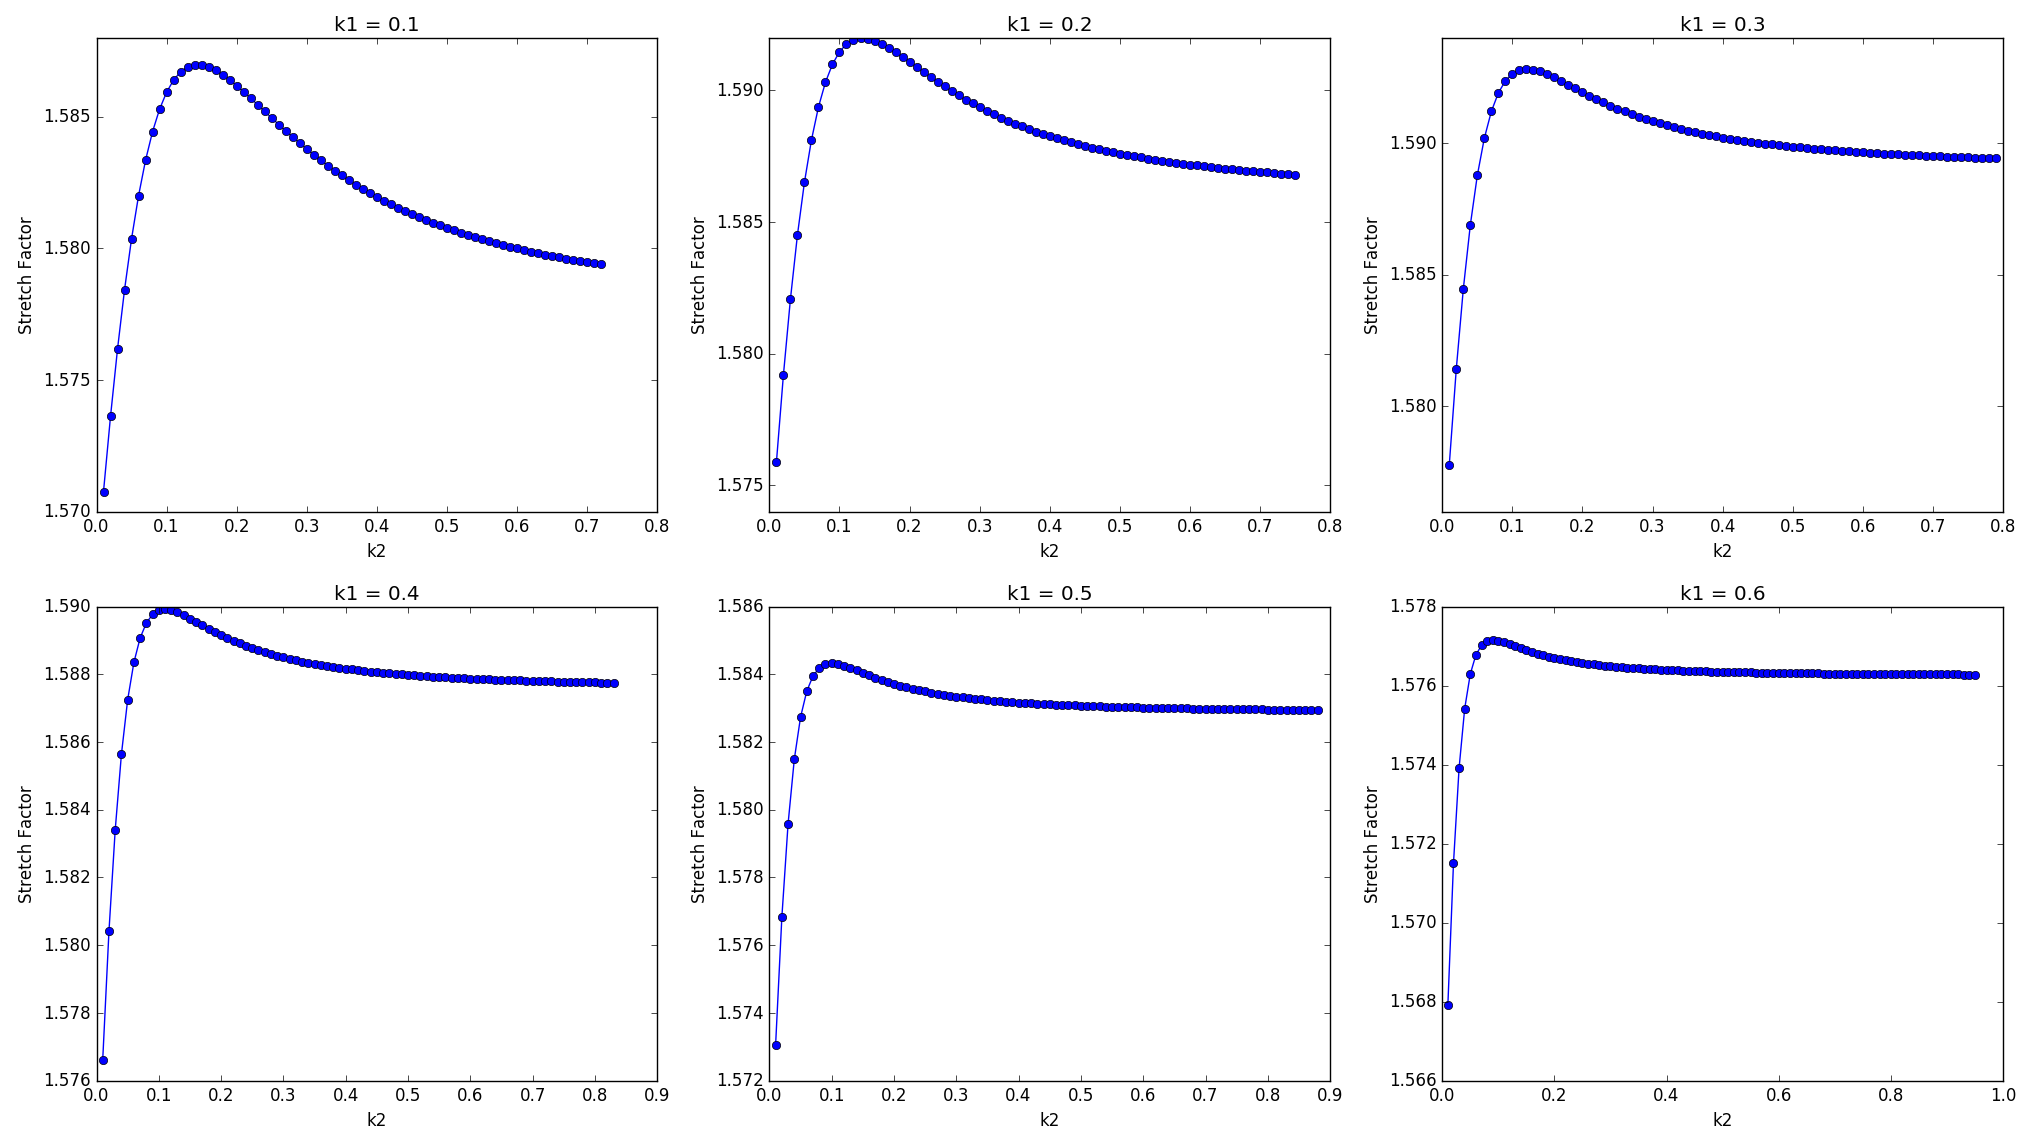
\includegraphics[width=\textwidth]{Figures/k1k2.png}
\caption[Constrained Delaunay triangulation in path planning in Automated driving]{Constrained Delaunay triangulation in path planning in Automated driving.} 
\label{fig:k1k2}
\end{figure}




\section{Study the Lower bound in Python}
As we discussed in Chapter 6, to improve the lower bound of the stretch factor in arcgons, we first calculate the partial derivatives in both $x$ and $k$ directions. Then, simulate recursively on the stretch factors of every block so that the maximun possible stretch factors based on the partial derivatives is still less than our target value, $1.6$. The following python code is our implementation of this simulation.
\begin{minted}[breaklines]{python}
from sympy import *

# Generate the partial derivatives of func f
x = Symbol('x');
k = Symbol('k');

path = 1.5707963267949 -asin(x) + sqrt(k**2+x**2)*atan(x/k)
distance = (sqrt(1-x**2)-k)*cos(x) + sqrt(k**2+x**2)*cos(x/sqrt(k**2+x**2)-x)
f = path/distance
diff_x = diff(f, x)
diff_k = diff(f, k)

print diff_x
print diff_k


# calculate the stretch factor given x and k
def func(x, k):
	path = 1.5707963267949 -asin(x) + sqrt(k**2+x**2)*atan(x/k)
	distance = (sqrt(1-x**2)-k)*cos(x) + sqrt(k**2+x**2)*cos(x/sqrt(k**2+x**2)-x)
	return path/distance

# find the partial derivative with respective to x
def pdiff_x(x, k):
	diff_x = (x*atan(x/k)/sqrt(k**2 + x**2) - 1/sqrt(-x**2 + 1) + sqrt(k**2 + x**2)/(k*(1 + x**2/k**2)))/((-k + sqrt(-x**2 + 1))*cos(x) + sqrt(k**2 + x**2)*cos(x - x/sqrt(k**2 + x**2))) + (sqrt(k**2 + x**2)*atan(x/k) - asin(x) + 1.5707963267949)*(x*cos(x)/sqrt(-x**2 + 1) - x*cos(x - x/sqrt(k**2 + x**2))/sqrt(k**2 + x**2) + (-k + sqrt(-x**2 + 1))*sin(x) + sqrt(k**2 + x**2)*(x**2/(k**2 + x**2)**(3/2) + 1 - 1/sqrt(k**2 + x**2))*sin(x - x/sqrt(k**2 + x**2)))/((-k + sqrt(-x**2 + 1))*cos(x) + sqrt(k**2 + x**2)*cos(x - x/sqrt(k**2 + x**2)))**2
	return diff_x

# find the partial derivative with respective to k
def pdiff_k(x, k):
	diff_k = (k*atan(x/k)/sqrt(k**2 + x**2) - x*sqrt(k**2 + x**2)/(k**2*(1 + x**2/k**2)))/((-k + sqrt(-x**2 + 1))*cos(x) + sqrt(k**2 + x**2)*cos(x - x/sqrt(k**2 + x**2))) + (sqrt(k**2 + x**2)*atan(x/k) - asin(x) + 1.5707963267949)*(k*x*sin(x - x/sqrt(k**2 + x**2))/(k**2 + x**2) - k*cos(x - x/sqrt(k**2 + x**2))/sqrt(k**2 + x**2) + cos(x))/((-k + sqrt(-x**2 + 1))*cos(x) + sqrt(k**2 + x**2)*cos(x - x/sqrt(k**2 + x**2)))**2
	return diff_k

# test if all maximun possible stretch factors is lower than the bound we give
def run(lb, rb, step, bound):
	ans = []
	delta_x = 0.739085/step
	delta_k = 1/step
	for i in range(step):
		x = 0.739085/step*(i+1)
		for j in range(step):
				k = 0.739085/step*(j+1)
				subans = [-1, -1, -1, -1, -1, -1]
				subans[0] = x
				subans[1] = k
				
				if k <= sqrt(1-x**2): 
					subans[2] = func(x, k)
					subans[3] = pdiff_x(x, k)*delta_x
					subans[4] = pdiff_k(x, k)*delta_k
					subans[5] = subans[2] - subans[3] - subans[4]

				ans.append(subans)
				if (subans[2]>bound or subans [5]>bound):
					# pass
					print "FAIL"
					run(lb, rb + step/2, step/2 , bound)
					print subans
					return subans
	print "SUCCESS"
	return ans

# run the program
ans = run(100, 1.6)

\end{minted}


% \clearpage
\printbibliography[heading=bibintoc, title={References}]



\end{document}
